% arara: xelatex
% arara: biber
% arara: xelatex: { synctex: true }


\documentclass[12pt,a4paper,oneside,final]{report}
\usepackage{tabularx}
\usepackage{float}
% \usepackage[russian]{babel}

\usepackage{tabularx}

\usepackage{polyglossia}
\setmainlanguage[numerals=cyrillic]{russian}
\setotherlanguages{english}
\usepackage{csquotes}

\usepackage{xunicode} % some extra unicode support
%\usepackage[utf8x]{inputenc}
\usepackage{xltxtra} % \XeLaTeX macro
\usepackage{fontspec}
\defaultfontfeatures{Ligatures=TeX}

%\setromanfont{Charis SIL}
%\setsansfont{Liberation Sans}
%\setmonofont{PT Mono}
%\setmainfont{Liberation Serif} % this allows to use sans-serif as default font

\usepackage{ifplatform}

\ifwindows
  \newfontfamily{\cyrillicfont}{Times New Roman}
  \setmainfont{Times New Roman}
  \newfontfamily{\cyrillicfonttt}{Courier New}
  \setmonofont{Courier New}
\else
  \setmainfont{Linux Libertine O}
  \setsansfont{Linux Biolinum O}
  \setmonofont[SmallCapsFont={Latin Modern Mono Caps}]{Latin Modern Mono Light}
\fi

%нумерация справа и колонтитулы справа вверху
\usepackage{fancyhdr}
\usepackage[a4paper,left=25mm,right=10mm,top=20mm,bottom=20mm,bindingoffset=0cm]{geometry}%

\usepackage{amsfonts}
\usepackage{amssymb}
\usepackage{amsmath}
\usepackage{amsthm}

\usepackage{calc}
\usepackage{ifthen}
\usepackage{graphicx}
\usepackage{array}
\usepackage{pdfpages}
\usepackage{longtable}
\usepackage{multirow}
\usepackage{indentfirst}
\usepackage[unicode=true]{hyperref}
\usepackage{color}
\usepackage{pgf}
\usepackage{pstheorems}
\usepackage{titling}

% Настройка списков (без лишних вертикальных отступов)
\usepackage{paralist}
\setdefaultenum{1.}{1.}{1.}{1.}
\setdefaultitem{--}{}{}{}
%\setlength\itemsep{-1em}
\let\itemize\compactitem
\let\enditemize\endcompactitem
\let\enumerate\compactenum
\let\endenumerate\endcompactenum
\let\description\compactdesc
\let\enddescription\endcompactdesc
\pltopsep=\smallskipamount
\plitemsep=0pt
\plparsep=0pt
% Команда для отмены разрыва страниц перед списками
\makeatletter 
\newcommand\mynobreakpar{\par\nobreak\@afterheading} 
\makeatother
%%%%%%

\usepackage[singlelinecheck=false,labelsep=endash]{caption}
\captionsetup[table]{justification=justified}
\captionsetup[figure]{justification=centering}

\usepackage{titlesec}
\titleformat{\chapter}[block]{\centering\normalfont\Large\bfseries}{\thechapter.}{1ex}{}{}
\titlespacing{\chapter}{0pt}{0em}{2em}

\titleformat{\section}[block]{\normalfont\large\bfseries}{\thesection}{1ex}{}{}
\titlespacing{\section}{0pt}{0em}{1ex}

\titleformat{\subsection}[block]{\normalfont\normalsize\bfseries}{\thesubsection}{1ex}{}{}
\titlespacing{\section}{0pt}{0em}{1ex}

	% paragraph и subparagraph -- в тексте, без отступов
\titleformat{\paragraph}[runin]{\normalfont\normalsize\bfseries}{\theparagraph}{0pt}{}{}
\titlespacing{\paragraph}{0pt}{0em}{0ex}

\titleformat{\subparagraph}[runin]{\normalfont\normalsize\bfseries}{\thesubparagraph}{0pt}{}{}
\titlespacing{\subparagraph}{0pt}{0em}{0ex}


% Своё название для Cписка литературы
\usepackage[title, titletoc]{appendix}
\addto\captionsrussian{% Replace "english" with the language you use
	\renewcommand{\contentsname}%
	{Содержание}%
}

%\renewcommand{\appendixname}{Приложение}% Change "chapter name" for Appendix chapters
%\renewcommand{\cftchapdotsep}{\cftdotsep}

\usepackage{mathpartir}

\makeatletter
\let\ps@plain\ps@fancy              % Подчиняем первые страницы каждой главы общим правилам
\makeatother
\pagestyle{fancy}
\fancyhf{}
\fancyfoot[C]{\thepage}
\renewcommand{\headrulewidth}{0pt}
\renewcommand{\footrulewidth}{0pt}
\renewcommand{\baselinestretch}{1.5}
\newcommand{\headertext}[1]{\fancyhead[R]{\tiny{#1}}}

%% Список литературы

\usepackage[
  style=gost-numeric,
  sorting=none,
  language=auto,
  autolang=other
]{biblatex}
\addbibresource{chapters/biblio.bib}

%\frenchspacing %% изменение расстояние до и после точек в ряде случаев

\renewcommand{\theenumi}{\arabic{enumi}}
\renewcommand{\theenumii}{\arabic{enumii}}
\renewcommand{\theenumiii}{\arabic{enumiii}}
\renewcommand{\theenumiv}{\arabic{enumiv}}

\renewcommand{\labelenumi}{\theenumi.}
\renewcommand{\labelenumii}{\theenumi.\theenumii.}
\renewcommand{\labelenumiii}{\theenumi.\theenumii.\theenumiii.}
\renewcommand{\labelenumiv}{\theenumi.\theenumii.\theenumiii.\theenumiv.}

%\newenvironment{annotation}{\textbf{Аннотация.} \textit}{}
\theoremstyle{plain}
\newtheorem*{annotation}{Аннотация}

\makeatletter
\newcommand*{\documenttype}[1]{\gdef\@documenttype{#1}}
\newcommand*{\thedocumenttype}{\@documenttype}
\newcommand*{\authorfulldative}[1]{\gdef\@authorfulldative{#1}}
\newcommand*{\theauthorfulldative}{\@authorfulldative}
\newcommand*{\authorgroup}[1]{\gdef\@authorgroup{#1}}
\newcommand*{\theauthorgroup}{\@authorgroup}
\newcommand*{\supervisor}[1]{\gdef\@supervisor{#1}}
\newcommand*{\thesupervisor}{\@supervisor}
\newcommand*{\consultant}[1]{\gdef\@consultant{#1}}
\newcommand*{\theconsultant}{\@consultant}
\makeatother

\newcounter{projecttasknumber}
\newcommand{\projecttask}{\setcounter{projectsubtasknumber}{0}\stepcounter{projecttasknumber}\theprojecttasknumber.}

\newcounter{projectsubtasknumber}
\newcommand{\projectsubtask}{\stepcounter{projectsubtasknumber}\theprojecttasknumber.\theprojectsubtasknumber.}

\usepackage{listings}

\renewcommand{\lstlistingname}{Листинг}

\lstset{
  basicstyle=\linespread{0.94}\ttfamily\small,
  tabsize=2,
  showstringspaces=false,
  columns=flexible,
  numbers=none,
  numberstyle=\tiny\color{gray},
  breaklines=true,
  breakatwhitespace=true,
  framesep=6pt,
  abovecaptionskip=1em,
  captionpos=b,
  extendedchars=true,
  inputencoding=utf8,
  literate={Ö}{{\"O}}1
  {Ä}{{\"A}}1
  {Ü}{{\"U}}1
  {ß}{{\ss}}1
  {ü}{{\"u}}1
  {ä}{{\"a}}1
  {ö}{{\"o}}1
  {~}{{\textasciitilde}}1
  {а}{{\selectfont\char224}}1
  {б}{{\selectfont\char225}}1
  {в}{{\selectfont\char226}}1
  {г}{{\selectfont\char227}}1
  {д}{{\selectfont\char228}}1
  {е}{{\selectfont\char229}}1
  {ё}{{\"e}}1
  {ж}{{\selectfont\char230}}1
  {з}{{\selectfont\char231}}1
  {и}{{\selectfont\char232}}1
  {й}{{\selectfont\char233}}1
  {к}{{\selectfont\char234}}1
  {л}{{\selectfont\char235}}1
  {м}{{\selectfont\char236}}1
  {н}{{\selectfont\char237}}1
  {о}{{\selectfont\char238}}1
  {п}{{\selectfont\char239}}1
  {р}{{\selectfont\char240}}1
  {с}{{\selectfont\char241}}1
  {т}{{\selectfont\char242}}1
  {у}{{\selectfont\char243}}1
  {ф}{{\selectfont\char244}}1
  {х}{{\selectfont\char245}}1
  {ц}{{\selectfont\char246}}1
  {ч}{{\selectfont\char247}}1
  {ш}{{\selectfont\char248}}1
  {щ}{{\selectfont\char249}}1
  {ъ}{{\selectfont\char250}}1
  {ы}{{\selectfont\char251}}1
  {ь}{{\selectfont\char252}}1
  {э}{{\selectfont\char253}}1
  {ю}{{\selectfont\char254}}1
  {я}{{\selectfont\char255}}1
  {А}{{\selectfont\char192}}1
  {Б}{{\selectfont\char193}}1
  {В}{{\selectfont\char194}}1
  {Г}{{\selectfont\char195}}1
  {Д}{{\selectfont\char196}}1
  {Е}{{\selectfont\char197}}1
  {Ё}{{\"E}}1
  {Ж}{{\selectfont\char198}}1
  {З}{{\selectfont\char199}}1
  {И}{{\selectfont\char200}}1
  {Й}{{\selectfont\char201}}1
  {К}{{\selectfont\char202}}1
  {Л}{{\selectfont\char203}}1
  {М}{{\selectfont\char204}}1
  {Н}{{\selectfont\char205}}1
  {О}{{\selectfont\char206}}1
  {П}{{\selectfont\char207}}1
  {Р}{{\selectfont\char208}}1
  {С}{{\selectfont\char209}}1
  {Т}{{\selectfont\char210}}1
  {У}{{\selectfont\char211}}1
  {Ф}{{\selectfont\char212}}1
  {Х}{{\selectfont\char213}}1
  {Ц}{{\selectfont\char214}}1
  {Ч}{{\selectfont\char215}}1
  {Ш}{{\selectfont\char216}}1
  {Щ}{{\selectfont\char217}}1
  {Ъ}{{\selectfont\char218}}1
  {Ы}{{\selectfont\char219}}1
  {Ь}{{\selectfont\char220}}1
  {Э}{{\selectfont\char221}}1
  {Ю}{{\selectfont\char222}}1
  {Я}{{\selectfont\char223}}1
  {…}{\ldots}1
  {–}{-}1
  {\ }{ }1
}

\authorgroup{М20-504}
\author{Клычков М. Д.}
\authorfulldative{Клычкову Матвею Дмитриевичу}
\supervisor{Самсонович А. В.}
\consultant{}


\headertext{}

\addto{\captionsrussian}{\renewcommand{\bibname}{Список литературы}}

%\title{Исследование и реализация сферического коня в вакууме\\
  %на основе теоретико-множественного подхода}

\title{Создание эмоционального искусственного интеллекта робота-пингвина}

\begin{document}

%\documenttype{Расширенное содержание пояснительной записки}
\documenttype{Пояснительная записка}

% Для титульного листа, сверстанного в LaTeX
\pagestyle{empty}
\begin{center}
  {\scriptsize
    \uppercase{Министерство науки и высшего образования российской федерации}\linebreak
    \uppercase{Федеральное государственное автономное образовательное
    учреждение высшего образования}
  }

  \textbf{Национальный исследовательский ядерный университет «МИФИ»}

  {\footnotesize
    \noindent\makebox[\linewidth]{\rule{\linewidth}{0.4pt}}
  }
\end{center}

\vskip 1em

\noindent
\begin{tabular}{@{}lc@{}}
\multirow{2}{*}{
\includegraphics[width=0.2\linewidth]{mephi.png}}
  & \textbf{\large{}Факультет Кибернетики и Информационной безопасности} \\
  & \uppercase{\textbf{\large{}Кафедра кибернетики (№ 22)}}  \\
\end{tabular}


\vfill

\begin{center}
  Направление подготовки 09.04.04 Программная инженерия

  \vfill

  {\Large{\textbf{\thedocumenttype}}}

  к научно-исследовательской работе студента на тему:

  {\Large\thetitle}
\end{center}

\vfill

{\large

\noindent
\begin{tabular}{@{}lcl@{}}
Группа              & $\rule{5cm}{0.15mm}$ & \theauthorgroup \\   
Студент             & $\rule{5cm}{0.15mm}$ & \theauthor \\    
Руководитель        & $\rule{5cm}{0.15mm}$ & \thesupervisor \\         
Научный консультант & $\rule{5cm}{0.15mm}$ & \theconsultant \\                
\end{tabular}

\vfill

\noindent
Оценка руководителя \quad $\rule{3cm}{0.15mm}$ \quad
Оценка комиссии     \quad $\rule{3cm}{0.15mm}$

\vfill

\noindent
\begin{tabular}{@{}lcc@{}}
Члены комиссии & & \\
& $\rule{6cm}{0.15mm}$ & $\rule{6cm}{0.15mm}$ \\
& $\rule{6cm}{0.15mm}$ & $\rule{6cm}{0.15mm}$ \\
& $\rule{6cm}{0.15mm}$ & $\rule{6cm}{0.15mm}$ \\
& $\rule{6cm}{0.15mm}$ & $\rule{6cm}{0.15mm}$ \\
\end{tabular}

\vfill

\begin{center}
\textbf{Москва \the\year}
\end{center}

}

\newpage

% Для вставки бланка титульного листа из PDF-файла
% \includepdf[pages={-}, offset=0mm -0mm]{title/title.pdf}

%\clearpage
%% Тут включается лист с подписями для ВКР
%\includepdf[pages={-}, offset=0mm -0mm]{title/title-dep22.pdf}
%\clearpage

% Для листа задания, сверстанного в LaTeX
\pagestyle{empty}
\begin{center}
  {\scriptsize
    \uppercase{Министерство науки и высшего образования российской федерации}\linebreak
    \uppercase{Федеральное государственное автономное образовательное
    учреждение высшего образования}
  }

  \textbf{Национальный исследовательский ядерный университет «МИФИ»}

  {\footnotesize
    \noindent\makebox[\linewidth]{\rule{\linewidth}{0.4pt}}
  }
\end{center}

\vskip 1em

\noindent
\begin{tabular}{@{}lc@{}}
\multirow{2}{*}{
\includegraphics[width=0.2\linewidth]{mephi.png}}
  & \textbf{\large{}Факультет Кибернетики и Информационной безопасности} \\
  & \uppercase{\textbf{\large{}Кафедра кибернетики (№ 22)}}  \\
\end{tabular}


\begin{center}
  {\Large{\textbf{Задание на НИР}}}

  \large
 
  Студенту гр. \theauthorgroup{} \theauthorfulldative
\end{center}

\begin{center}
  \uppercase{\textbf{\large{}Тема НИР}}

  {\Large\thetitle}

  \vskip 1em

  \uppercase{\textbf{\large{}Задание}}
\end{center}

{\linespread{1.0}
  \footnotesize
  \noindent
  \begin{longtable}{|p{.5cm}|p{250pt}|>{\centering\arraybackslash}p{2cm}|>{\centering\arraybackslash}p{2cm}|>{\centering\arraybackslash}p{2cm}|} \hline
  \multicolumn{1}{|>{\centering\arraybackslash}p{0.5cm}|}{№\par п/п} & \multicolumn{1}{c|}{Содержание работы} & Форма отчетности & Срок исполнения & Отметка о выполнении\par {\scriptsize Дата, подпись} \\\hline
\projecttask & Аналитическая часть &&& \\\hline
% (указываются предмет и цели анализа)
\projectsubtask & Изучение и анализ классических математических моделей Земли и способов нахождения кратчайших расстояний на них
  & Пункт ПЗ
  &
  &
  \\\hline
\projectsubtask & Изучить материалы описывающие движение воздушного судна
  & Пункт ПЗ
  &
  &
  \\\hline
\projectsubtask & Изучение и анализ теории компьютерной графики применительно к построению полигональных сеток
  & Пункт ПЗ
  &
  &
  \\\hline
\projectsubtask & Анализ методов компьютерной графики применительно
к задачам построения заданных кривых в пространстве
  & Пункт ПЗ
  &
  &
  \\\hline
%\projectsubtask & Анализ методов нахождения пересечений кривых и полигональных сеток в трехмерном пространстве
  %& Пункт ПЗ
  %&
  %&
  %\\\hline
\projectsubtask & Оформление расширенного содержания пояснительной записки (РСПЗ) & Текст РСПЗ & 10.10.2021 & \\\hline%
\projecttask & Теоретическая часть &&& \\\hline
% (указываются используемые и разрабатываемые модели, методы, алгоритмы)
\projectsubtask & Аффинное преобразование
  &
  &
  &
  \\\hline
\projectsubtask & Описание математической модели Земли
  & Модели
  &
  &
  \\\hline
\projectsubtask & Разработка алгоритмов построения полигональной сетки на основе таблицы высот земной поверхности
  & Алгоритмы
  &
  &
  \\\hline
\projectsubtask & Разработка алгоритмов построения траектории движения воздушного судна
  & Алгоритмы
  &
  &
  \\\hline
\projectsubtask & Модификация методов аппроксимации компьютерной графики для построения траектории движения воздушного судна
  & Алгоритмы
  &
  &
  \\\hline
\projecttask & Инженерная часть &&& \\\hline
% (указывается, что конкретно необходимо спроектировать, а также используемые для этого методы, технологии и инструментальные средства)
\projectsubtask & Проектирование методов и алгоритмов компьютерной графики, адаптированных под задачу построения полигональной модели Земли
  & Макеты
  &
  &
  \\\hline
\projectsubtask & Проектирование классов и функций, для расчёта траектории движения воздушного судна
  & Макеты
  &
  &
  \\\hline
\projectsubtask & Проектирование классов и функций, для нахождения пересечения кривых и полигональной сетки
  & Макеты
  &
  &
  \\\hline
\projectsubtask & Проектирование юнит-тестов для проверки корректности работы статической библиотеки
  & Макеты
  &
  &
  \\\hline
\projectsubtask & Результаты проектирования оформить с помощью UML диаграмм
  & UML диаграммы
  &
  &
  \\\hline
\projecttask & Технологическая и практическая часть &&& \\\hline
% (указывается, что конкретно должно быть реализовано и протестировано, а также используемые для этого методы, инструментальные средства, технологии)
\projectsubtask & Реализация статической библиотеки адаптированных методов и алгоритмов компьютерной графики, для построения полигональной сетки
  & Исполняемые файлы, исходный текст 
  &
  & \\\hline%
\projectsubtask & Реализация статической библиотеки адаптированных методов и алгоритмов компьютерной графики, для построения траектории воздушного судна
  & Исполняемые файлы, исходный текст 
  &
  & \\\hline%
\projectsubtask & Реализация статической библиотеки адаптированных методов и алгоритмов компьютерной графики, для нахождения пересечения траектории воздушного судна и земной поверхности
  & Исполняемые файлы, исходный текст 
  &
  & \\\hline%
\projectsubtask & Тестирование статической библиотеки адаптированных методов и алгоритмов компьютерной графики
  & Исполняемые файлы, исходные тексты тестов и тестовых примеров
  &
  &
  \\\hline
\projecttask & Оформление пояснительной записки (ПЗ) и иллюстративного материала для доклада. & Текст ПЗ, презентация & 01.01.2022 & \\\hline
\end{longtable}
}
%\refsection
%\nocite{Sychev}
%\nocite{Sokolov}
%\nocite{Gaidaenko}
%\begin{center}
  %\uppercase{\textbf{\large{}Литература}}
%\end{center}
%\printbibliography[heading=none]
%\endrefsection

\begin{center}
  \uppercase{\textbf{\large{}Литература}}
\end{center}

\begin{itemize}
  \item Никулин Е. А. Компьютерная геометрия и алгоритмы машинной графики. — СПб: БХВ-2. Петербург, 2003
  \item Эдвард Энджел. Интерактивная компьютерная графика. Вводный курс на базе OpenGL = Interactive Computer Graphics. A Top-Down Approach with Open GL. — 2-е изд. — : «Вильямс», 2001
  %\item Колесников К. С. Динамика ракет / К. С. Колесников. – М. : Машиностроение, 2003
  %\item Абгарян К. А. Динамика ракет / К. А. Абгарян, И. М. Рапопорт. – М. : Машиностроение, 1969
  \item Ефремов А.В., Захарченко В.Ф., Овчаренко В.Н., Суханов В.Л. Динамика полета: учебник для студентов высших учебных заведений – М. : Машиностроение, 2011
  \item Bjarne Stroustrup The C++ Programming Language Special Edition. - М.: Издательство «БИНОМ» 2012
  \item Andrew Koenig, Barbara E. Moo Accelerated C++: Practical Programming by Example.
\end{itemize}


\vfill

{\noindent\linespread{2.0}
  \begin{tabularx}{\linewidth}{p{140pt}XXX}
    Дата выдачи задания: & Руководитель & \hrulefill & \theauthor \\
    10.10.2021           & Студент      & \hrulefill & \thesupervisor \\
  \end{tabularx}
}


% Для вставки бланка задания из PDF-файла
%\includepdf[pages={-}, offset=0mm -0mm]{title/zadanie.pdf}
\newpage

\pagenumbering{arabic}

\refsection

%\clearpage
%\thispagestyle{empty}

%\vfill

%\begin{center}
%[Место для распечатки отчета Антиплагиата]
%\end{center}

%\newpage
%\thispagestyle{empty}

%\vfill

%\begin{center}
%[Место для распечатки отчета Антиплагиата]
%\end{center}

\clearpage

\chapter*{Реферат}
\thispagestyle{plain}


Пояснительная записка содержит 46 страниц, 19 рисунков, ~-- 32 источников литературы.

Ключевые слова: UNITY3D, EBICA, СОЦИАЛЬНО-ЭМОЦИОНАЛЬНЫЙ ИНТЕЛЛЕКТ, ВИРТУАЛЬНЫЙ АКТОР, МАШИННОЕ ОБУЧЕНИЕ, РЕККУРЕНТНЫЕ СЕТИ 

Объектом исследования являются экспертные системы.

Предмет исследования - модель когнитивной архитектуры для создания Виртуального Актора.

Целью данной научно-исследовательской работы является создание прототипа Виртуального Актора, 
модель интеллекта которого основана на когнитивной архитектуре eBICA.
Существует два глобальных подхода к созданию социально-эмоционального интеллекта. 
Один основанный на нейросетях, другой на когнитивных архитектурах.
В ходе работы над НИР был разработан и протестирован с участием испытуемых прототип Виртуального Актора, 
обладающий социально-эмоциональным интеллектом и помещенный в виртуальное окружение, которое создано при помощи графического движка Unity3d, 
была реплизована сиетема для анализа речи с выявлением эмоций соответствующим речевым признакам, так же были
в дополнении к вышеуказанной системе, были спроектированы и реализованы методы 
воздействия на виртуального агента, основыющиеся на семантичекой составляющей речевого контекста.
Данная работа является актуальной поскольку на данный момент эта область находится на начальных этапах 
развития и активной интеграции в различные индустрии.
Созданная и протестированная модель интеллекта затем может быть интегрирована в другие проекты с 
Виртуальным Актором: виртуальный слушатель, виртуальный клоун, виртуальный танцор. 





\clearpage

\tableofcontents{}

\clearpage

\chapter*{Введение}
\label{sec:afterwords}
\addcontentsline{toc}{chapter}{Введение}


В последнее время все большую и большую популярность набирают технологии предоставляющие возможность участвовать человеку 
в виртуальном мире либо технические средства, позволяющие представление виртуальную реальность в реальном мире.
Виртуальные Акторы способны в будущем заменить докладчика на конференциях различного характера и представлениях,
быть интегрированы в процесс обучения студентов, быть использользованы как развивающие игрушки для детей.
Однако, до сих пор не существует реализованной модели, которая представляет из себя полноценный эмоциональный интеллект.

Вдобавок, даже в настоящем взайимодействие человека и машины становится буквально повседневным и может во многом
в будущем упростить жизнь людей. К примеру примненением для системы взаимодействия робота и человека может быть 
выражено посредсвом их вербального общения, такое взаимодействие может быть полезно для оказания помощи немощным людям. 
Технология распознающая эмоции может отслеживать эмоциональное состояние человека для выявления аномалий в его поведении. 
Когда возникает аномалия, это может означать, что человек требует внимания.

Кроме того, распознавание эмоций может быть практичным в диагностике некоторых заболеваний 
(депрессивные расстройства, болезнь Паркинсона,
и т.д.) 
выявлением дефицита выражения определенных эмоций, ускорением диагноз, так и лечение потенциального пациента.


Целью данной научно-исследовательской работы является создание прототипа Виртуального Актора с многомодальным интерфейсом, 
модель интеллекта которого основана на когнитивной архитектуре eBICA.
Существует два глобальных подхода к созданию социально-эмоционального интеллекта. 
Один основанный на нейросетях, другой на когнитивных архитектурах.
В ходе работы над ВКР был разработан и протестирован прототип Виртуального Актора, 
обладающий социально-эмоциональным интеллектом и помещенный в виртуальное окружение, которое создано при помощи графического движка Unity3d, 
была реализована система для анализа речи с выявлением эмоций соответствующим речевым признакам, так же были
в дополнении к вышеуказанной системе, были спроектированы и реализованы методы 
воздействия на виртуального агента, основывающиеся на семантической составляющей речевого контекста.
Данная работа является актуальной поскольку на данный момент эта область находится на начальных этапах 
развития и активной интеграции в различные индустрии.
Созданная и протестированная модель интеллекта затем может быть интегрирована в другие проекты с 
Виртуальным Актором: виртуальный слушатель, виртуальный клоун, виртуальный танцор. 



\clearpage

\chapter{Исследование существующих когнитивных архитектур и анализ их недостатков}


Проводится анализ по выявлению существующих недоработок прототипа. 
Выявляются недостатки и преимущества по сравнению с другими моделями искусственного интеллекта.

%Это обзорно-аналитическая глава, в которой требуется отразить:

%\begin{itemize}
	%\item результат изучения различных существующих методов решения задач в рамках проблематики УИРа/диплома (иногда даже в смежных областях), это обзорный аспект, который пишется, в основном, на основе имеющейся литературы или/и программного обеспечения;
	%\item сравнение (с какой-либо определенной целью) этих методов и средств.
%\end{itemize}

%Приведенные ниже названия пунктов являются очень примерными, их состав и структура сильно зависят от специфики конкретной работы.




%Большие отсупы --- это хорошо. Облегчает чтение длинных <<простыней>> текста


%ок
\section{Изучение и анализ существующих когнитивных архитектур}

Одной из наиболее известных когнитивных архитектур является архитектура, 
составленная Jonathan Gratch и Stacy Marsella, что описано в работе \cite{Samsonovich03}.
Цель их исследования - создать общую вычислительную модель механизмов, 
лежащих в основе человеческих эмоций, которая сможет всецело их описать. 
Хотя такая модель может давать объяснение человеческого поведения, 
они рассматривают разработку вычислительных моделей эмоций как 
ключевой объект исследований для искусственного интеллекта, 
который будет способствовать развитию большого количества вычислительных систем,
которые моделируют, интерпретируют или влияют на человеческое поведение. 
На рисунке (Рис. \ref{pic:ris1}) демонстрируется Когнитивно-мотивационно-эмоциональная система.

\begin{figure}[h]
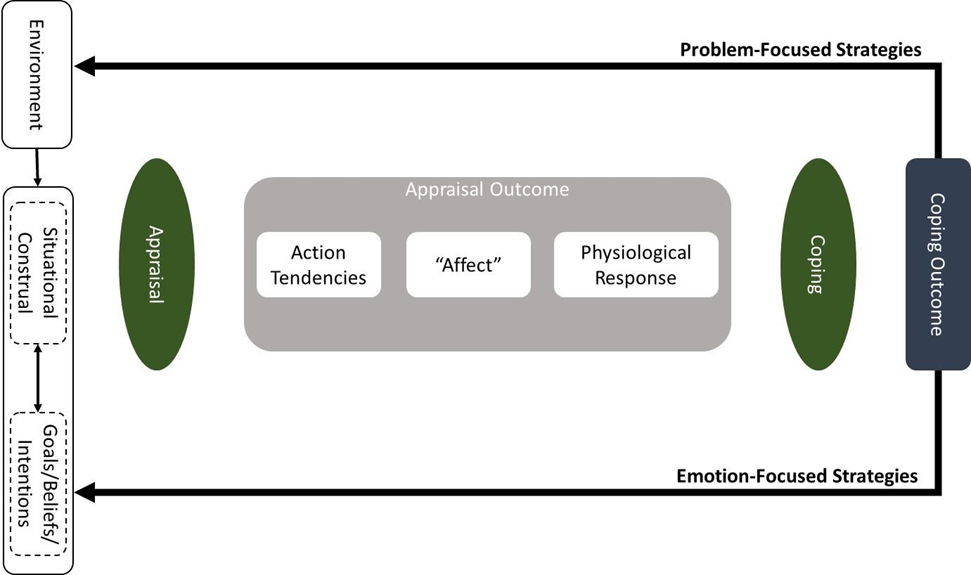
\includegraphics[width=0.75\columnwidth]{./img/ris1.png}
\centering
\caption{Когнитивно-мотивационно-эмоциональная система по материалам Smith and Lazarus.}
\label{pic:ris1}
\end{figure}

Теория оценки служит концептуальной основой их работы, но эта психологическая теория недостаточно точна, чтобы служить
спецификацией вычислительной модели. Для этого они переделывают теорию с точки зрения методов и представлений искусственного интеллекта. 
Когнитивно-мотивационно-эмоциональная система Craig Smith и Richard Lazarus, показанная на рисунке 1, является представителем современных
теорий оценки. Эмоция концептуализируется как двухступенчатая система контроля. Оценка характеризует отношения между человеком и его 
физическим и социальным окружением, называемые отношениями человека и окружающей среды, копирование поведения для восстановления или 
поддержания этих отношений. Поведение возникает в результате тесной связи познания, эмоций и реакций совладения: когнитивные процессы 
служат для построения индивидуальной интерпретации того, как внешние события соотносятся с его целями и желаниями 
(отношения человека и окружающей среды). Система использует эти характеристики для изменения отношений между человеком и окружающей средой,
мотивируя действия, которые изменяют среду (копирование, ориентированное на проблему), или мотивируя изменения в интерпретации этих 
отношений (копирование, ориентированное на эмоции).

Модель PAD была разработана Albert Mehrabian и James A. Russell в 1974 году для описания и измерения эмоциональных состояний, как говорится в Работе \cite{Samsonovich04}. 
В данной модели используются три числовых измерения для представления всех эмоций:
\begin{itemize}
	\item A — arousal (возбуждение);
	\item P — pleasure (удовольствие); 
	\item D — dominance (доминирование).
\end{itemize}

Модель PAD первоначально использовалась в теории психологии окружающей среды, а основное идеей модели было предположение о том,
что физическая среда влияет на людей через их эмоциональное воздействие. На основе данной модели были построены физиологическая 
теория эмоций и теория эмоциональных эпизодов. Также модель использовалась для изучения невербального общения, в потребительском 
маркетинге и при создании анимированных персонажей, которые выражают эмоции.

В модели PAD используются трехмерные шкалы, которые в теории могут иметь любые числовые значения:
\begin{itemize}
	\item шкала удовольствия-неудовольствия показывает, насколько приятно или, наоборот, неприятно человек себя чувствует по отношению к чему-то. Например, радость это — приятная эмоция; гнев и страх — неприятные эмоции;
	\item шкала возбуждения-неактивности измеряет, насколько человек чувствует возбуждение или его отсутствие. В данном случае оценивается именно возбуждение, а не интенсивность эмоций. Например, горе или депрессия характеризуются слабым возбуждением, но сильной интенсивностью; а гнев или ярость имеют и высокую интенсивность, и высокое состояние возбуждения;
	\item шкала доминирования-покорности описывает чувство контроля и доминирования по сравнению со смирением и подчиненностью. Например, гнев — это доминирующая эмоция, а страх
	\item эмоция покорности, хотя обе они имеют неприятный характер.
	\item эмоция покорности, хотя обе они имеют неприятный характер.
\end{itemize}

Еще одна интересная когнитивная архитектура описана в статье трех научных деятелей Ron Sun, Nick Wilson, 
Michael Lynch. Статья имеет название: “Emotion: A Unified Mechanistic Interpretation from a Cognitive Architecture”.
В этой статье рассматривается проект, который пытается интерпретировать эмоции - сложное и многогранное явление с 
механистической точки зрения, чему способствует существующая комплексная вычислительная когнитивная архитектура - CLARION.
Эта когнитивная архитектура состоит из ряда подсистем: подсистем, ориентированных на действие, не ориентированных надействия, 
мотивационной и метакогнитивной подсистем. С этой точки зрения эмоции в первую очередь основаны на мотивации.
Основываясь на этих функциональных возможностях, мы механистически (вычислительно) соединяем части вместе 
в рамках CLARION и фиксируем множество важных аспектов эмоций, как описано в литературе. 
На (Рис. \ref{pic:ris2}) демонстрируются подсистемы когнитивной архитектуры CLARION.
\begin{figure}[h]
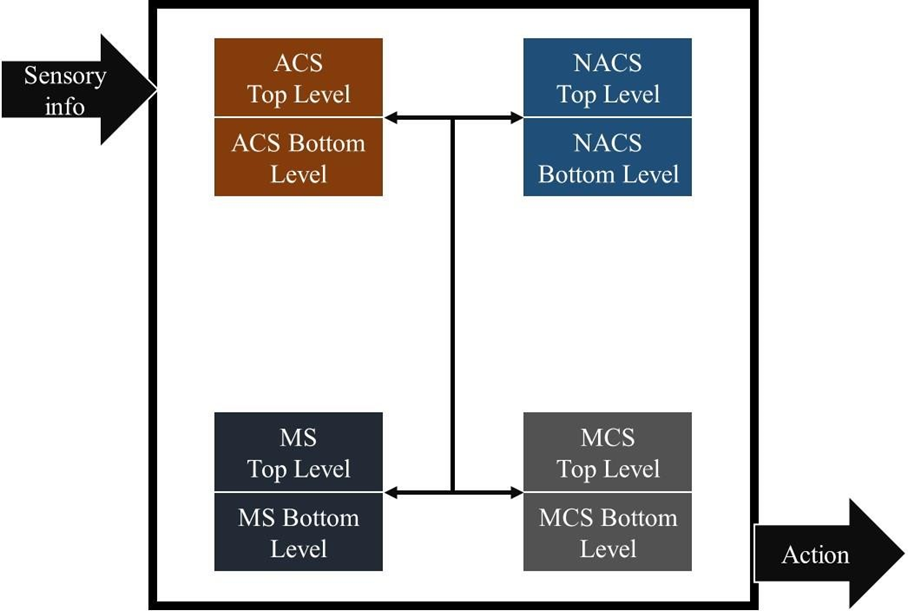
\includegraphics[width=0.75\columnwidth]{./img/ris2.png}
\centering
\caption{Подсистемы когнитивной архитектуры CLARION}
\label{pic:ris2}
\end{figure}

Основные информационные потоки показаны стрелками. ACS означает подсистему, ориентированную на действия. NACS означает подсистему, не ориентированную на действия. МС — это мотивационная подсистема. MCS означает метакогнитивную подсистему.

Получившая наибольшее распространение из всех формальных моделей представления эмоций является модель OCC (Ortony, Clore, \& Collins), 
которая упоминается в работет \cite{Samsonovich06}, 
предложенная в 1988 году учеными Кембриджского университета. Иерархия содержит три ветви, а именно: эмоции, касающиеся последствий 
событий (например, радость и жалость), действия агентов (например, гордость и упрек) и аспекты объектов (например, любовь и ненависть). 
Кроме того, некоторые ветви объединяются в группу сложных эмоций, а именно эмоций относительно последствий событий, вызванных действиями 
агентов (например, благодарность и гнев). 
На рисунке (Рис. \ref{pic:ris3}) демонстрируется оригинальная модель OOC.

\begin{figure}[h]
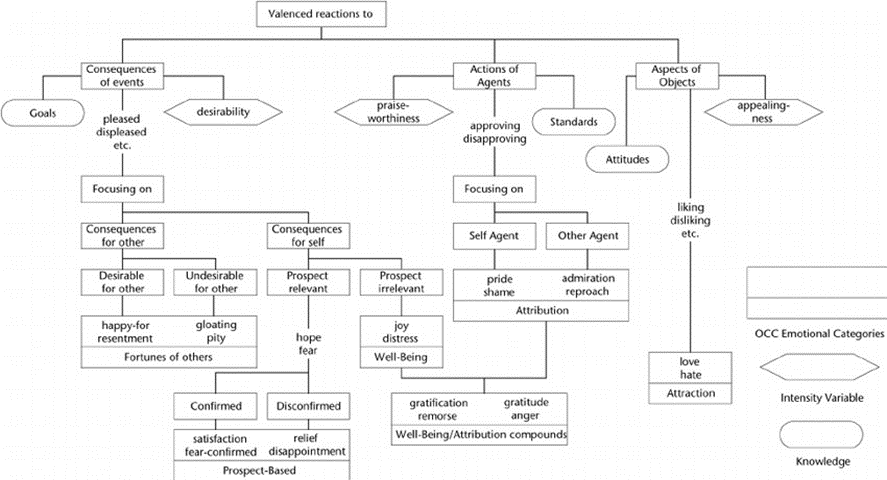
\includegraphics[width=0.75\columnwidth]{./img/ris3.png}
\centering
\caption{Оригинальная модель OCC}
\label{pic:ris3}
\end{figure}
В основе правил динамики данной модели лежит реакция валентности (Valenced reaction). 
Под «валентностью» в психологии понимают внутреннюю привлекательность – «хорошую» 
(положительную валентность) или отвратительность – «плохую» (отрицательную валентность) 
события, объекта или ситуации. Эмоции формируются под воздействием трех основных факторов — 
последствий событий (Consequences of events), действий движущих сил (Actions of agents) и аспектов событий.

Рассмотрим левую «ветку» эмоциональной реакции. Последствия событий могут быть приносящими 
удовольствие (pleased) или доставляющими неудовольствие (displeased). Проведя предварительную 
оценку, человек фокусируется (Focusing on) на разделении последствий событий для себя 
(Consequences for self) и для других (Consequences for self), которые, в свою очередь могут 
оказаться для последних желательными (Desirable for other) или нежелательными (Undesirable for other). 
По поводу судеб других (Fortunes of others) в зависимости от личного отношения — положительного или 
отрицательного — человек может испытывать следующие эмоции: радость за другого (Happy for), 
обида (Resentment), злорадство (Gloating) или жалость (Pity).

У этой модели есть свои ограничения, заключающиеся как в ее требовании упрощения человеческих эмоций,
 так и в ее сложном подходе к тому, как надлежит выводить эмоциональные состояния конечных пользователей 
 посредством интерпретации поведения человека через знаки и сигналы, транслируемые людьми. Использование 
 этой модели в ее оригинальном описании затруднено отсутствием математического аппарата, в следствии чего 
 многие исследователи в своих Виртуальных Акторах используют упрощённые версии данной модели.

Также большой интерес представляет когнитивная архитектура, реализованная в физическом роботе, 
под названием - интегрированное когнитивное универсальное тело (iCub). Это когнитивная архитектура,  
дизайн которой  основан на  существующих знаниях в области робототехники, вычислений, нейробиологии и 
психологии, целью которой является копирование некоторых когнитивных процессов человека для их включения 
в человекоподобных роботов.

Эта архитектура реализована в человекоподобном роботе. Он был разработан для исследования сообществом когнитивных систем. 
Кроме того, он имеет лицензию «Стандартная общественная лицензия GNU (GPL)», так что любой человек может свободно использовать 
все наработки по данному проекту. Данная архитектура реализована в человекоподобном роботе, который имеет 53 степени свободы. 
По размеру он похож на ребенка трех-четырех лет и ребенка в возрасте 2,5 лет по когнитивным способностям. Кроме того, он может 
ползать и сидеть. Некоторые особенности, которые описаны в работе \cite{Samsonovich02}

\begin{itemize}
	\item	Не хватает семантической памяти, чтобы помочь ему обобщать события;
	\item Невозможно сформировать привычки;
	\item Он учится путем подражания, проб и ошибок;
	\item Обнаруживает, распознает и отслеживает человеческое лицо, наблюдая за его действиями; 
	\item Действия основаны на жестах рук, таких как встряхивание и манипулирование объектами,например, толкание, подъем и опускание. 
	\item Действия, наблюдаемые роботом, изучаются и сохраняются в базе данных в процессе обучения.
\end{itemize}

На рисунке (Рис. \ref{pic:ris4}) представлена схема работы iCub.
\begin{figure}[h]
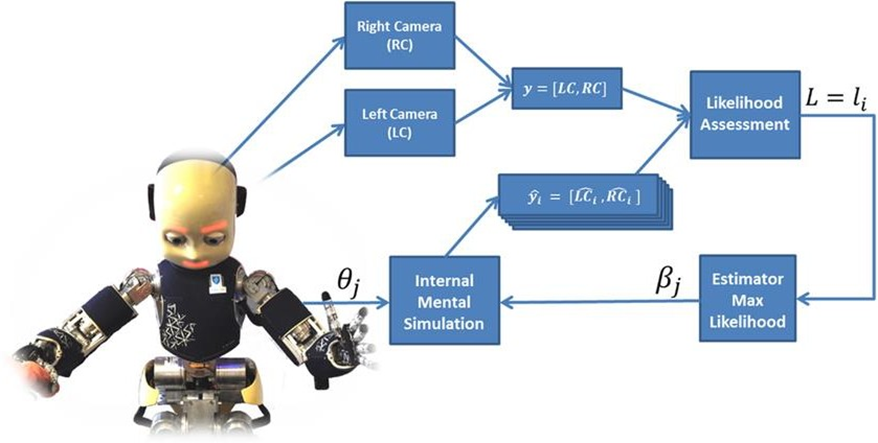
\includegraphics[width=0.75\columnwidth]{./img/ris4.png}
\centering
\caption{Схема работы iCub}
\label{pic:ris4}
\end{figure}

Вспомогательным инструментом при создании актора, наделенного социально- эмоциональным интеллектом, 
может являться - имитация моторного обучения (IML). IML начинает наблюдать за другим актором, осуществляющим 
некоторую цепочку действий, затем категоризирует действия (определяет какую цель преследуют данные действия) 
одновременно отслеживая изменения точки обзора, окружающей среды, положения и типов объектов. Другими словами, 
когда Виртуальный агент неоднократно наблюдает за определенной новой последовательностью действий, каждый из 
знакомых элементов действия активирует соответствующее моторное представление через существующие ассоциации. 
Данное наблюдение формирует связи между элементарными моторными представлениями. Эта связь представлений 
составляет моторное обучение и улучшает имитационное движение. Способность моторной системы интегрировать 
разные части организма позволила бы создать обширный репертуар моторного поведения путем смешивания выходных 
сигналов разных частей организма, чтобы конечный результат отражал относительный и взвешенный вклад каждого в 
достижении цельной имитации движения. Поскольку невозможно воспроизвести функционирование мозга, были созданы 
модели, которые пытаются имитировать различные функции и поведение.
%ок
\section{Изучение и анализ когнитивной архитектуры eBICA}

Архитектура состоит из семи компонентов: интерфейсный буфер, рабочая, процедурная, семантическая 
и эпизодическая системы памяти, система ценностей и система когнитивных карт. Три основных строительных 
блока для этих компонентов — это ментальные состояния, схемы и семантические карты. 
Семантическая память — это коллекция определений схем. Буфер интерфейса заполняется схемами. 
Рабочая память включает активные психические состояния. Эпизодическая память хранит неактивные психические состояния,
сгруппированные в эпизоды - предыдущее содержимое рабочей памяти. Следовательно, эпизодическая память состоит из структур, 
аналогичных тем, которые обнаруживаются в рабочей памяти, но которые «заморожены» в долговременной памяти \cite{seman_karta}. Процедурная 
память включает в себя примитивы. Система ценностей включает в себя шкалы, представляющие основные значения. 
Система когнитивных карт включает, в частности, семантические карты эмоциональных ценностей. 
Семантическая карта использует абстрактное метрическое пространство (семантическое пространство) для представления
семантических отношений между ментальными состояниями, схемами и их 13 экземплярами, а также для присвоения значений их оценкам. 
На (Рис.\ref{pic:ris5}) демонстрируется семантическая карта \cite{seman_karta}.

\begin{figure}[h]
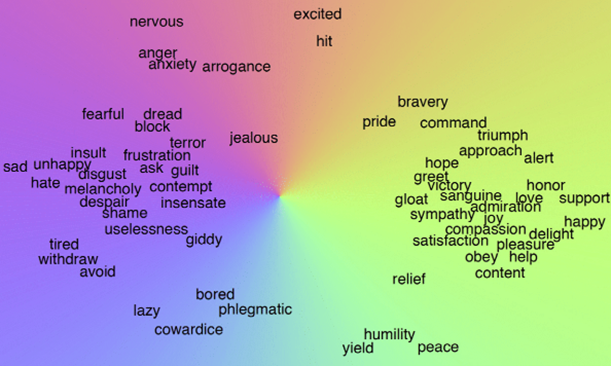
\includegraphics[width=0.75\columnwidth]{./img/ris5.png}
\centering
\caption{Семантическая карта}
\label{pic:ris5}
\end{figure}

Для когнитивного семантического отображения может использоваться слабое когнитивное семантическое картирование. 
Идея заключается в том, чтобы расположить представления на основе очень немногих основных семантических измерениях. 
Эти измерения могут возникать автоматически, если стратегия состоит в том, чтобы объединить синонимы и антонимы друг от друга. 
Карта, часть которой показана на рисунке 6 является результатом этого процесса. Эта карта не очень хорошо отделяет различные 
значения друг от друга: например, основные и сложные чувства. Однако она классифицирует значения в соответствии с их семантикой. 
Рисунок (Рис. \ref{pic:ris6}) демонстрирует примеры простейших эмоциональных элементов в рамках eBICA \cite{Samsonovich01}.

\begin{figure}[h]
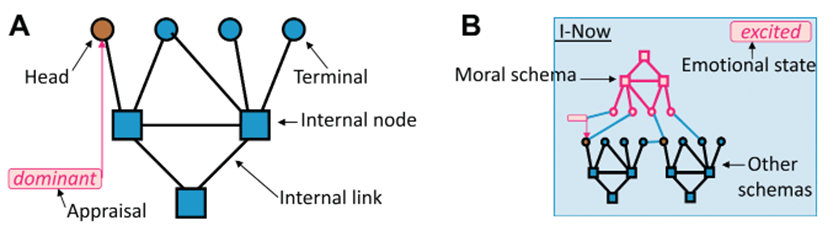
\includegraphics[width=0.75\columnwidth]{./img/ris6.png}
\centering
\caption{примеры эмоциональных элементов в рамках eBICA}
\label{pic:ris6}
\end{figure}

(A) Схема имеет оценку в качестве своего атрибута. Это также атрибут головного узла. Значение этого атрибута - «доминантный», 
что означает, что действие воспринимается как проявление доминирования, или агент воспринимается как «доминантный по отношению ко мне» 
и т. Д. (B) Психическое состояние имеет оценку атрибут, который представляет собой эмоциональное состояние и самооценку агента в данный 
момент в данной ментальной перспективе. Показанная ценность этой оценки «взволнована», что означает, что агент находится в возбужденном 
эмоциональном состоянии. Моральная схема, показанная в B, связывается с частью содержания психического состояния (включая определенный 
образец оценок) и представляет оценку выбранного образца, например, образец взаимодействий и взаимных оценок двух агентов, упомянутых в 
ментальном состоянии.

%можно еще дописать
\section{Нейронные сети и их типы}

Нейро́нная сеть (также искусственная нейронная сеть, ИНС) — математическая модель, а также её программное или аппаратное воплощение, 
построенная по принципу организации и функционирования биологических нейронных сетей — сетей нервных клеток живого организма. 
Это понятие возникло при изучении процессов, протекающих в мозге, и при попытке смоделировать эти процессы. Первой такой попыткой 
были нейронные сети У. Маккалока и У. Питтса. После разработки алгоритмов обучения получаемые модели стали использовать в практических 
целях: в задачах прогнозирования, для распознавания образов, в задачах управления и др. 

Разделяют несколько основных разновидностей Нейронных сетей, согласно работе \cite{neural01}, а именно:
\begin{itemize}
	\item Нейронные сети прямого распространения
	\item Сети радиально-базисных функций
	\item Нейронная сеть Хопфилда (Hopfield network, HN)
	\item Цепи Маркова (Markov chains, MC или discrete time Markov Chains, DTMC)
	\item Машина Больцмана (Boltzmann machine, BM)
	\item Ограниченная машина Больцмана (restricted Boltzmann machine, RBM)
	\item Автокодировщик (autoencoder, AE)
	\item Разреженный автокодировщик (sparse autoencoder, SAE)
	\item Вариационные автокодировщики (variational autoencoder, VAE)
	\item Шумоподавляющие автокодировщики (denoising autoencoder, DAE)
	\item Сеть типа «deep belief» (deep belief networks, DBN)
	\item Свёрточные нейронные сети (convolutional neural networks, CNN)
	\item Развёртывающие нейронные сети (deconvolutional networks, DN)
\end{itemize}

С точки зрения машинного обучения, нейронная сеть представляет собой частный случай методов распознавания образов, дискриминантного анализа.
Рекуррентные нейронные сети (РНС, англ. Recurrent neural network; RNN) — вид нейронных сетей, где связи между элементами образуют 
направленную последовательность \cite{Wikipedia01}. Благодаря этому появляется возможность обрабатывать серии событий во времени или последовательные 
пространственные цепочки. В отличие от многослойных перцептронов, рекуррентные сети могут использовать свою внутреннюю память для 
обработки последовательностей произвольной длины. Поэтому сети RNN применимы в таких задачах, где нечто целостное разбито на части, 
например: распознавание рукописного текста или распознавание речи. Было предложено много различных архитектурных решений для 
рекуррентных сетей от простых до сложных. В последнее время наибольшее распространение получили сеть с долговременной и 
кратковременной памятью (LSTM) и управляемый рекуррентный блок (GRU).

В последнее время наибольшую популярность для решения задач тематической классификации, применяемой для выделения семантического смысла текста,
приобрели глубокие нейронные сети, так как они позволяют достичь наивысшей точности среди всех известных моделей машинного обучения. 
В частности, сверточные нейронные сети совершили прорыв в классификации изображений. В настоящее время они успешно справляются и с 
некоторыми задачами автоматической обработки текстов. Более того, как утверждается в некоторых исследованиях сверточные сети подходят 
для этого даже лучше рекуррентных нейронных сетей, которые чаще всего используются для анализа текстовых последовательностей. 
С другой стороны, использование сверточных сетей для классификации текстов мало исследовано. Поэтому исследование применения 
сверточных нейронных сетей для задачи классификации текстов в качестве альтернативы рекуррентным нейронным сетям представляет 
практический интерес, что описано в \cite{neural10}.

Для решения поставленной задачи требуется получить способ представления данных в виде, пригодном для обработки сверточной нейронной сетью. 
Например, в виде матрицы вещественных чисел. Наиболее распространенным является способ отображения каждого слова в многомерное 
векторное пространство. В рамках данной работы векторные представления слов строились на основе модели word2vec \cite{cyberlinka01}.
sa

\section{Методы определения эмоций в речи}

Для распозавнания эмоций в речи используют следующие подходы:
\begin{itemize}
	\item Анализ эмотивной сотсавляющей текста в речи
	\item Анализ тональности речи
\end{itemize}


На текущий момент сущестуют следующие методы определения тональности текста:
\begin{enumerate}
  \item Анализ текста методами векторного анализа (часто с применением n-граммных моделей), сравнение с ранее размеченным эталонным корпусом по выбранной мере близости и отнесение (классификация) текста к негативу или позитиву на основании полученного результата сравнения.
  \item Поиск эмотивной лексики (лексической тональности) в тексте по заранее составленным тональным словарям (спискам паттернов) с применением лингвистического анализа. По совокупности найденной эмотивной лексики текст может быть оценен по шкале, отражающей количество негативной и позитивной лексики. Этот метод может использовать как списки паттернов, подставляемые в регулярные выражения, так и правила соединения тональной лексики внутри предложения
  \item Смешанный метод (комбинация первого и второго подходов).
\end{enumerate}

% тут надо нормально проставить cit
Первый метод (см., например, [Pang & al., 2002; Pang & al., 2005; Gamon,
2004]) работает достаточно быстро, но требует наличия предварительно размеченного эталонного корпуса, на основе которого происходит обучение алгоритма сравнения. 
Существенными недостатками такого подхода оказываются увеличение трудоемкости и ограничение разнородности корпуса (т. е.
неполнота лексического покрытия), что приводит к потере точности. К тому же
данный метод не позволяет провести глубокий анализ текста, то есть выявить
и показать эмотивность на уровне предложения.
% тут надо нормально проставить cit

Второй метод [Nasukawa, 2003; Yi, 2003] не менее трудоемок в составлении тональных словарей (или получения списка тональных паттернов),
Метод определения эмоций в текстах на русском языке 513
но в сочетании с синтаксическим и морфологическим анализом более гибок:
он позволяет не только показать цепочки тональной лексики, но и получить
синтаксически корректные эмоциональные выражения. При хорошем наполнении тональных словарных списков этот метод позволяет достичь хорошей
полноты (покрытия эмотивной лексики).
% тут надо нормально проставить cit
Недостаток этого метода в том, что с помощью него сложно дать количественную оценку негативности-позитивности текста. 
Чтобы избежать недостатков первого и второго метода, используют смешанный подход [Prabowo &
al., 2009; Konig, 2006], частично включающий в себя два первых.

Следующий метод определения эмоций в речи это их распознавание, посредством акустического анализа.

Индивидуальность голоса обеспечивается сочетанием поведенческих и
физиологических признаков. К поведенческим относят семантику, дикцию,
произношение, ритм, интонации и др. Они обусловлены социальными факто-
рами и могут быть довольно изменчивыми в зависимости от ситуации. Более
надежными являются анатомические особенности речевого тракта, поэтому
для работы автоматического распознавания наиболее адаптированы алгорит-
мы измерения акустических характеристик.

Акустическая теория речи рассматривает речевую волну как результат ра-
боты источника звука и фильтров. Подробное изложение о физиологических
процессах речеобразования и моделях речевого тракта можно найти в кни-
гах [2–4]. Здесь же кратко приведены только те параметры, которые участву-
ют в автоматическом распознавании дикторов.
Характерные черты голоса конкретного человека в цифровой обработке
сигналов получают через спектральный анализ речевой волны.

Частота первой гармоники спектра является частотой основного тона
(основной частотой голоса). Частота основного тона F0 – обратная величина
длительности T0 одного цикла работы голосовых связок: F0 = 1/ T0 . Основная
частота определяет высоту голоса – ощущение, связанное с воздействием тона
на слуховую систему человека.
Индивидуальность данного параметра объясняется тем, что длительность
T0 зависит от массы и упругости голосовых связок, а также от перепада дав-
ления над и под связками. Поэтому пол и возраст диктора оказывают влияние
на значения основной частоты.
Каждый человек имеет свой диапазон изменений частоты основного тона.
Как правило, для взрослого он составляет от полутора до двух октав. В задаче
распознавания личности по голосу необходимо определять базовую основную
частоту, т. е. привычный и удобный для идентифицируемого человека режим
работы голосовых связок.

\section{Классификации и определение эмоций}

Многообразие эмоций, их качественных и количественных проявлений исключают возможность простой и единой классификации. 
Каждая из характеристик эмоций может выступать в качестве самостоятельного критерия, основания для их классификации (таб. \ref{tbl:text_a00}).

\begin{table}[H]
\caption{характеристики эмоции как основания для их классификации}
\label{tbl:text_a00}
\begin{center}
%\centering

\begin{tabular}{ | c | c | }
	\hline
	Знак & Пололожительные, отрицательные, амбивалентные \\ \hline 
	Модальность & Радость, гнев, страх и др. \\ \hline
	Влияение на поведение и деятельность & Осознаваемые, неосознаваемые \\ \hline
	Предметность	& Предметные, беспредментные \\ \hline
	Степень произвольности & Произвольные, непроизвоольные \\ \hline
	Происхождение и развлечения & Врожденные, приобретенные, первичные, вторичные \\ \hline
	Уровень & Высшие, низшие \\ \hline
	Длительность & Кратковременные, длительные \\ \hline
	Интенсивность & Слабые, сильные \\ \hline
\end{tabular}
\end{center}
\end{table}

По знаку эмоциональные переживания можно разделить:
\begin{enumerate}
	\item на положительные
	\item отрицательные
	\item амбивалентные
\end{enumerate}

Основной функцией положительных эмоций является поддержание контакта с позитивным событием, поэтому им присуща реакция приближения к полезному, 
необходимому стимулу. Кроме того, по мнению П.В. Симонова, они побуждают нарушать достигнутое равновесие с окружающей средой и искать новую стимуляцию.

Для отрицательных эмоций характерной является реакция удаления, прерывания контакта с вредным или опасным стимулом.
Считается, что они играют более важную биологическую роль, поскольку обеспечивают выживание индивида.

Амбивалентными эмоциями являются противоречивые эмоциональные переживания, связанные с двойственным отношением к чему-либо или кому-либо (одновременное принятие и отвержение).

\section{Выводы}

Были изучены и проанализированы основные когнитивные архитектуры, особое внимание уделялось когнитивной архитектуры eBICA.
Была рассмотрена проблема синтеза и распознавание речи. Были изучены материалы описывающие классификацию и определение эмоций.



\clearpage

\chapter{Описание моделей, отвечающих за генерацию поведения виртуального актора}


В данном разделе приводится теоретическое описание модели.

\section{Постановка задачи}
% тут описать то что обсуждали с А.В.
В рамках научно-исследовательской работы был расширен подход решения поставленной задачи задачи, который выражается в
использовании машинного обчучения. Данный подход используется в совокупности когнитивной архитектурой eBICA. 
eBICA – “emotional biologically inspired cognitive architecture” – “эмоциональная биологически вдохновленная когнитивная архитектура”. 

В этой архитектуре эмоциональные элементы добавлены практически ко всем процессам за счет модификации основных строительных блоков архитектуры. 
Ключевым моментом этой когнитивной архитектуры являются оценки, которые связаны со схемами и психическими состояниями как их атрибуты, 
моральные схемы, которые контролируют модели оценок и представляют социальные эмоции, а также семантические пространства, которые дают 
значения этих оценок.

Как видно из (Рис. \ref{pic:ris7}), архитектура представляет собой конгломерат компонентов: интерфейсный буфер, рабочая, процедурная, семантическая 
и эпизодическая системы памяти, система ценностей и система когнитивных карт \cite{Samsonovich01}. Три основных строительных блока для этих компонентов - это 
ментальные состояния, схемы и семантические карты. Семантическая память - это коллекция определений схем. Буфер интерфейса заполняется схемами.

\begin{figure}[h]
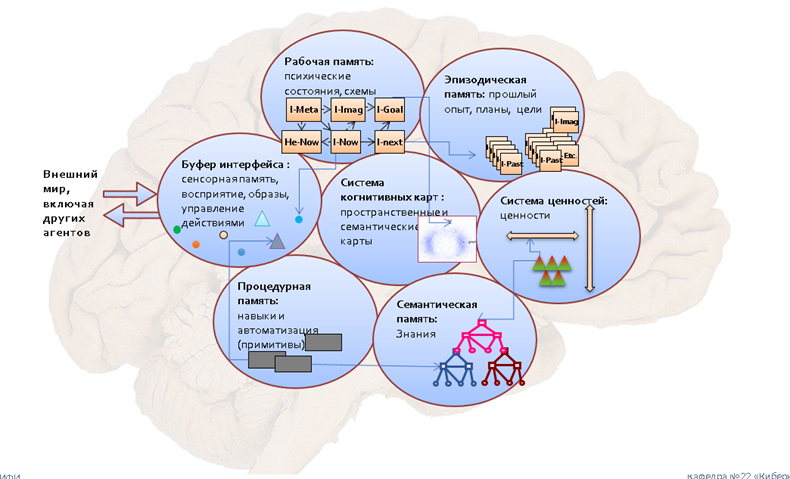
\includegraphics[width=0.75\columnwidth]{./img/ris7.png}
\centering  
\caption{Структура когнитивной архитектуры eBICA}
\label{pic:ris7}
\end{figure}

Рабочая память включает активные психические состояния. Эпизодическая память хранит неактивные психические состояния, сгруппированные 
в эпизоды - предыдущее содержимое рабочей памяти. Следовательно, эпизодическая память состоит из структур, аналогичных тем, которые 
обнаруживаются в рабочей памяти, но которые «заморожены» в долговременной памяти. Процедурная память включает в себя примитивы. Система 
ценностей включает в себя шкалы, представляющие основные значения. Система когнитивных карт включает, в частности, семантические карты 
эмоциональных ценностей. Семантическая карта использует абстрактное метрическое пространство (семантическое пространство) для представления 
семантических отношений между ментальными состояниями, схемами и их экземплярами, а также для присвоения значений их оценкам.


\section{Описание работы модели актора}

На момент начала выполнения работы уже была реализована система работы виртуальных агентов, и она состоит в том, что сперва 
считываются действия и объекты с заданными для них параметрами и значениями из Excel файла, а также инициализируются значения. 
Затем выбор действий происходит в следующем порядке: в радиусе вокруг оценок виртуального актора выбираются действия, которые 
попадают в этот радиус, а также проверяются различные условия, необходимые для выполнения действия. Если условия не выполняются, 
то действие не может быть выбрано. Затем, после того как в список добавлены все действия, которые могут быть выполнены, рассчитываются 
вероятности на основе оценок и рассчитанных констант. Также, если действие повторное, его вероятность несколько занижается. 
После расчета вероятностей выбирается действие, которое влияет на оценки виртуального актора. 

Помимо этого происходит замена состояний объектов и виртуальных акторов. После этого происходит перерасчет оценок Appraisals и Feelings \cite{Samsonovich01}.

Основная модель eBICA определяет поведение виртуального актора исходя из следующих факторов:

\begin{itemize}
  \item соматический;
  \item рациональный;
  \item когнитивный.
\end{itemize}

Нравственный фактор регулирует отношения первого актора со вторым на основе системы ценностей (представленной семантической картой) 
и моральных схем. Под когнитивным фактором понимается учет соображений нравственности, этики и морали, общей системы ценностей, 
понятий о добре и зле, о собственном достоинстве, эмпатии, соображений эстетики, стремлений к простоте и элегантности, и т.д. 
Учет этих соображений возможен на основе когнитивных оценок (appraisals) всех релевантных агентов, событий, их возможных действий 
и последствий этих действий, фактов, свойств, отношений, и т.д. Возможен вариант модели, в которой ответное действие может выбираться 
лишь из двух вариантов: положительная реакция на действие человека и отрицательная. Данная версия модели весьма неплохо работает даже 
с таким ограничением. Но невозможно придерживаться данной парадигмы при увеличении количества возможных вариантов для взаимодействия 
между акторами. В данной модели необходимо учесть пересчет оценок Appraisals и Feelings. Для пересчета оценок Appraisals используется 
следующая формула \ref{eq:appraisals01}:

\begin{equation}
  \begin{gathered}
    Appraisals=(1-r)*Appraisals+r*Action
    %P_{i+1j  } (R_{i+1j  } , {\varphi}_{i+1} , {\theta}_{j  }) \\
  \end{gathered}
  \label{eq:appraisals01}
\end{equation}

где Appraisals - оценка, 
r - эмпирически вычисленная константа экспоненциального затухания, 
Action - оценка совершаемого действия на семантической карте.

Одновременно с Appraisals пересчитываются так называемые “чувства” Feelings согласно режиму работы моральной схемы.
Аффективное пространство VAD – это трехмерное векторное пространство, точки которого соответствуют определенным эмоциональным 
состояниям, или аффектам, представленным триплетами значений (Valence, Arousal, Dominance). 
Существуют и сходные модели: PAD (Pleasure, Arousal, Dominance), EPA (Evaluation, Potency, Arousal) и другие. 
Здесь мы используем модель VAD. Соответственно, под «семантической картой» здесь часто понимается ее конкретная 
разновидность: аффективная карта (или когнитивная семантическая карта).

Шкалы имеют следующие значения:
\begin{itemize}
  \item dominance – варьируется при значении от 0 (покорность) до +1 (доминантность) и описывает соответствующие чувства; 
  \item valense – при значениях от -1 до 0 показывает уровень негатива или радости соответственно; 
  \item arousal – значения от -1 до 1 показывают уровень возбуждения (заинтересованности), к примеру, гнев по уровню возбуждения сильнее раздражительности, но слабее ярости. 
\end{itemize}

Оценки представлены в виде векторов на трехмерной семантической карте \cite{seman_karta}, \ref{pic:ris5}.
Моральная схема определяет общую установку на оценку поведения акторов, согласно их ролям и типу ситуации. 
Ее целью (как агента) является достижение и поддержание «нормального» положения дел, определенного набором Feelings. 
Вообще говоря, моральная схема состоит из двух частей: части, распознающей тип ситуации и осуществляющей привязку (binding),
и части, реализующей динамику схемы. В случае парадигмы актора можно считать, что моральная схема одна, уже привязана, и 
потому первая часть ее не актуальна.

Субъективные оценки (Feelings) генерируются по определенным правилам на основании истории объективных оценок и состояний системы. 
Грубо говоря, Feelings – это субъективное представление о том, каким оцениваемый актор является «на самом деле», и, следовательно, 
какого поведения от него нужно ожидать и на какое место его нужно ставить своим поведением. Следовательно, выбор поведения актора 
должен осуществляться так, чтобы приблизить Appraisals к Feelings. 

Значение Feelings определяет моральная схема, которая может работать в одном из трех режимов. 
Первый режим основывается на формуле \ref{eq:feelings01}:

\begin{equation}
  \begin{gathered}
    Feelings=beta*Appraisals
  \end{gathered}
  \label{eq:feelings01}
\end{equation}

где beta – эмпирически вычисленная константа. 

В данном режиме схема говорит, что если актор ведет себя хорошо, то к нему нужно относиться как к хорошему, и т.д. 

Цель данного процесса – распознать и классифицировать актора, выработать отношение к нему и приписать ему определенную роль во взаимоотношениях. 

В данном режиме моральная схема работает пока разница между квадратами норм Feeling и Appraisals не станет меньше некоторого значения.

Суть второго режима заключается в том, что значение Feeling фиксировано и экстремально по абсолютной величине, т.е. находится на сфере, 
ограничивающей семантическую карту (предположим, что есть такая сфера). Направленность вектора Feeling может быть либо произвольной, 
определенной предысторией, либо дискретной – вдоль одной из осей.

Третий режим состоит в том, что значения Feelings меняются \ref{eq:feelings02}, подстраиваясь под текущие значения Appraisals (здесь r1 может быть отличным от r): 

\begin{equation}
  \begin{gathered}
    Feelings=(1-r_1 )*Feelings+r1*(Appraisal-Feelings)
  \end{gathered}
  \label{eq:feelings02}
\end{equation}

Соответственно значения Appraisals и Feelings как говорится в работе \cite{Samsonovich05} пересчитываются после каждого действия первого актора, направленного на второго актора.
Также пересчет оценок происходит после определения и совершения одним из акторов ответного или самостоятельного действия. 
В данном контексте под термином “самостоятельное действие” имеется в виду действие, основанное лишь на текущем состоянии мира и 
значений векторов Appraisals и Feelings акторов, отобрежнные на (Рис. \ref{pic:ris8}). 


\begin{figure}[h]
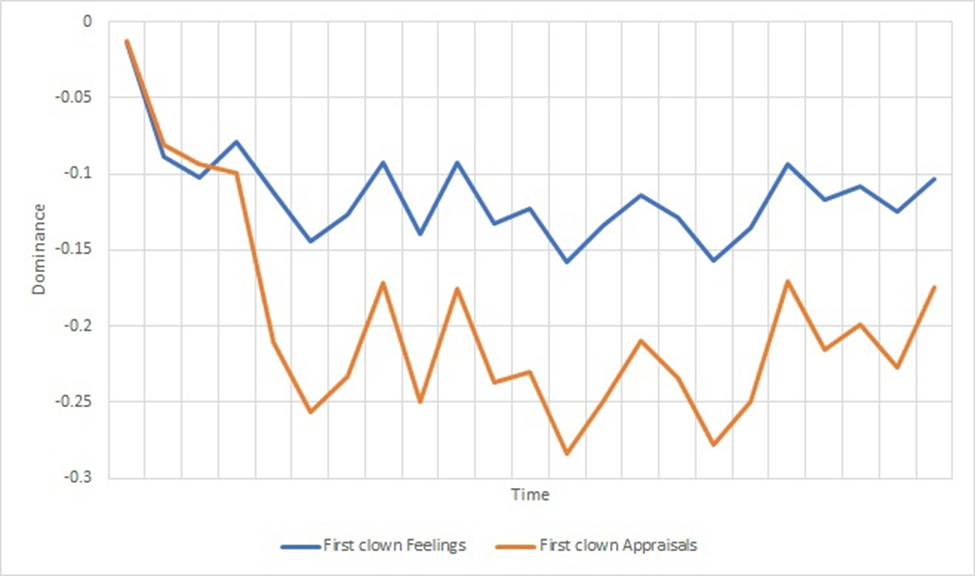
\includegraphics[width=0.75\columnwidth]{./img/ris8.png}
\centering
\caption{Корреляция значений Appraisals (оранжевая) и Feelings (синяя) для показателя доминантности на протяжении времени/действий с шагом в 5 секунд}
\label{pic:ris8}
\end{figure}

Согласно (Рис. \ref{pic:ris8}) мы видим, что работа модели сводится к выбору действия, 
которое будет максимально приближать Appraisals к Feelings и вектор соматического состояния к начальному положению.

\section{Способы распознавания речи}
Сейчас существует несколько методов решения задачи распознавания речи в аудиозаписи. Успешность и скорость их работы во многом зависит от дикции автора, качества записи аудиофайла, поданного на вход, фонового шума, а также от качества работы спроектированной системы распознавания, и, как следствие, от выбранного метода.

Разнообразие особенностей речи, а также реализуемых подходов к решению задачи распознавания ведут к многообразию существующих решений. Все они борются за лидерство по качеству работы, но все еще имеют свои индивидуальные достоинства и недостатки.

Самыми популярными методами распозвавания речи являются: 
\begin{itemize}
  \item Скрытое Марковское моделирование (HMM)
  \item Использование N-грамм
  \item Подход искусственного интеллекта
  \item Рекуррентные сети
\end{itemize}

До сих пор наиболее успешный \cite{1_speach} и часто используемый метод для распознавания речи - это математическая модель, полученная на основе модели Маркова (Рис. \ref{pic:speach_1}).
Скрытая Марковская модель представляет собой статистическую модель, моделирующую процесс Маркова с неизвестными параметрами. Пусть имеет N состояний модели. 
Каждое из состояний имеет свою вероятность наступления. Обозначим вероятности перехода между состояний как матрицу A=\{aij\}, где aij – вероятность перехода из i-го в j-е9
состояние. В каждом из своих состояний система принимает одно из M значений какого-то своего параметра. 

Обозначим вероятность выпадения каждого из M значений параметра в каждом из N состояний системы через B=\{bj(k)\}, 
где bj(k) – вероятность выпадения k-го значения параметра в j-м состоянии. Также введем вектор вероятности наступления начального состояния через 
π=\{πi\}, где πi – вероятность того, что в начальный момент система окажется в i-м состоянии. На рисунке \ref{pic:speach_1} представлена схема строения скрытой Марковской модели. 
Состояния представлены в виде голубых кружков (N штук), значения скрытого параметра представлены с помощью желтых квадратов (M штук). 
Каждая стрелка символизирует возможный переход и имеет свой вес (значение вероятности). Таким образом, скрытой Марковской моделью называется тройка λ = \{A, B, π\} \cite{2_speach}.

\begin{figure}[h]
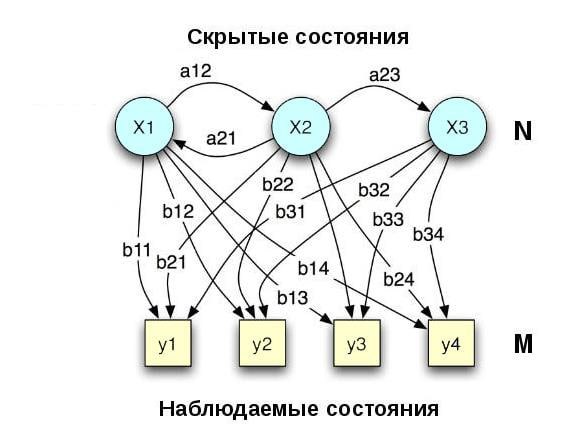
\includegraphics[width=0.75\columnwidth]{./img/speach_1.jpg}
\centering
\caption{Общая схема устройства скрытой Марковской модели. \cite{3_speach}}
\label{pic:speach_1}
\end{figure}

Использование скрытых Марковских моделей для распознавания речи основано на трех допущениях \cite{4_speach}:
\begin{enumerate}
  \item речь можно разбить на фрагменты (соответствующие состояниям в СММ) так, что внутри каждого фрагмента речевой сигнал можно рассматривать как стационарный. Параметры речи в его пределах постоянны;
  \item переход между состояниями осуществляется мгновенно;
  \item вероятность каждого фрагмента зависит только от текущего состояния модели и не зависит от предыдущих состояний.
\end{enumerate}

N-грамма – это модель представления данных, которая также может использоваться для распознавания речи \cite{5_speach}. 
N-граммная модель рассчитывает вероятность последнего элемента N-граммы при условии, что известны все предыдущие. 
В задаче распознавания речи элементами могут выступать фонемы, если задача решается на более низком уровне, или же целые слова. 

При использовании этого подхода предполагается, что появление каждого слова (фонемы) зависит только от предыдущих слов (фонем),
причем значение N указывает, от скольких предыдущих слов оно зависит. 


Вероятность фразы можно вычислить как произведение вероятностей каждого из слов этой фразы:

\begin{equation}
  \begin{gathered}
  P=P(мой) \times P(дядя|мой) \times P(самых|мой дядя) \times P(честных|мой дядя самых) \times P(правил|мой дядя самых честных)
  \end{gathered}
  \label{eq:speach_formula_1}
\end{equation}

Здесь $P(самых|мой дядя)$ обозначает условную вероятность возникновения «самых» при условии появления «мой дядя». Чтобы определить $P(мой)$, нужно посчитать, сколько раз это слово встретилось в тексте, и поделить это значение на общее число слов. 
Рассчитать вероятность $P(правил|мой дядя самых честных)$ уже сложнее. Чтобы упростить эту задачу, примем, что вероятность слова в тексте зависит только от предыдущего слова. Именно здесь проявляет себя выбранное значение N. 
Тогда формула для расчета фразы примет вид:

\begin{equation}
  \begin{gathered}
    P = P(мой) \times P(дядя|мой) \times P(самых|дядя) \times P(честных|самых) \times P(правил|честных)
  \end{gathered}
  \label{eq:speach_formula_2}
\end{equation}

Рассчитать условную вероятность $P(дядя|мой)$ несложно. Для этого считаем количество пар 'мой дядя', и делим на количество в тексте слова 'мой'. 
В результате, если мы посчитаем все пары слов в некотором тексте, мы сможем вычислить вероятность произвольной фразы. 
Этот набор рассчитанных вероятностей и будет биграммной моделью. Степень модели указывает на количество слов, учитываемых при расчете вероятностей. 
Рисунок \ref{pic:speach_2} показывает несколько N-грамм для небольших значений N. Униграмма имеет степень 1, биграмма – степень 2, триграмма – степень 3.

\begin{figure}[h]
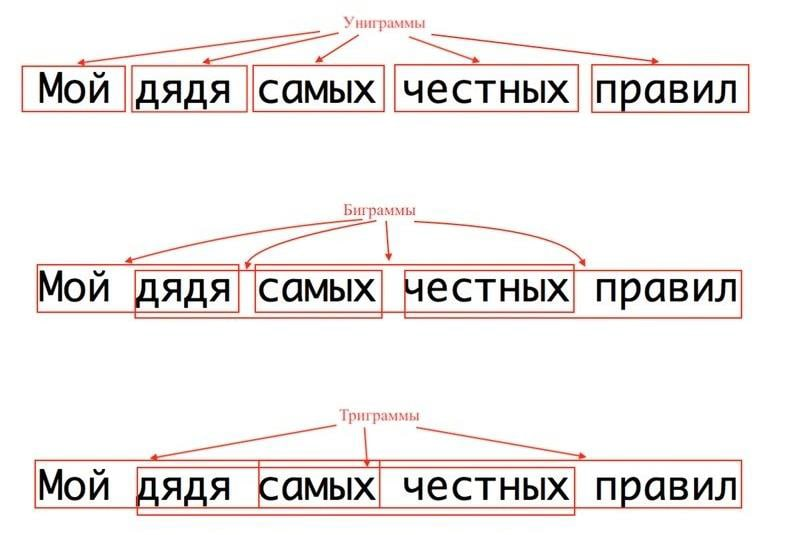
\includegraphics[width=0.75\columnwidth]{./img/speach_2.jpg}
\centering
\caption{N-грамма для N=1,2,3}
\label{pic:speach_2}
\end{figure}  

Представим фразу w как последовательность слов $w = (w1,w2,w3,…,wk)$. 
Тогда более формально N-граммная модель рассчитывает вероятности по формуле:

\begin{equation}
  \begin{gathered}
    p(w) = \prod_{i=1}^{k+1}p(w_{i}|w_{i-1})
  \end{gathered}
  \label{eq:speach_formula_3}
\end{equation}

\begin{equation}
  \begin{gathered}
    w_{i-n+1}^{i-1} = (w_{i-n+1}, ..., w_{i-1})
  \end{gathered}
  \label{eq:speach_formula_4}
\end{equation}

Тогда формула вычисления вероятностей биграммы представляется в виде:

\begin{equation}
  \begin{gathered}
    w_{i-n+1}^{i-1} = (w_{i-n+1}, ..., w_{i-1})
  \end{gathered}
  \label{eq:speach_formula_5}
\end{equation}

Подход с использованием методов машинного обучения один из самых часто используемых подходов. 
Для этого используют: 
\begin{itemize}
  \item Рекуррентные сети
  \item Двунаправленные рекуррентные сети
  \item Свёрточная нейронная сеть
\begin{itemize}

Рекуррентные нейронные сети (RNN) - это класс нейронных сетей, обладающих искусственной внутренней памятью. 
Такие сети используются в случаях, когда важна сама последовательность данных и та временная динамика, которая соединяет данные. 
Последовательные данные – это, в основном, просто упорядоченные данные, в которых связанные объекты следуют друг за другом. 
Примерами могут служить тексты, финансовые данные, последовательность ДНК, или данные временных рядов. Различные архитектуры 
рекуррентных сетей позволяют работать с разной необходимой глубиной памяти, в следствие чего спектр задач, в которых такие сети 
могут применяться, достаточно велик. Возможность учитывать порядок входных данных делает рекуррентные сети идеально подходящими 
для задач машинного обучения, связанных с обработкой текстовых данных.

В RNN информация проходит циклически и с каждым циклом может затухать – запоминать более новую информацию, обновляя память. 
Когда принимается решение, сеть учитывает текущие входные данные, а также то, что она узнала на предыдущих слоях. \
Рисунок \ref{pic:recur} иллюстрирует разницу в потоке информации между RNN и обычной нейронной сетью.

\begin{figure}[h]
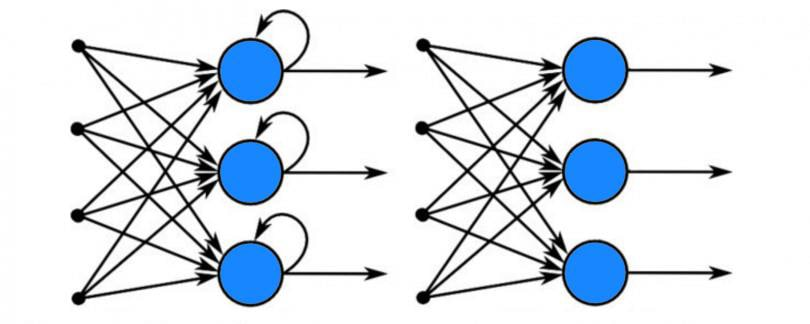
\includegraphics[width=0.75\columnwidth]{./img/recur.jpg}
\centering
\caption{Сравнение структуры рекуррентной нейронной сети (справа) и cети прямого распространения (слева). \cite{recur}}
\label{pic:recur}
\end{figure}

Нейроны сети производят вывод, а также копируют этот вывод и зацикливают его обратно на свой вход.
Так они получают информацию не только от предыдущего слоя, но и от самих себя предыдущего прохода. 
Это означает, что порядок, в котором подаются данные и обучается сеть, становится важным.

Большой проблемой при работе сетей RNN является проблема исчезающего градиента, которая заключается в быстрой потере информации с течением времени. 
Сети способны хранить только самую недавнюю информацию, что не всегда является достаточным для данной задачи. 
Допустим, мы хотим предсказать последнее слово в тексте “Я вырос в России… Мой родной язык русский”. 
Ближайший контекст предполагает, что последним словом будет называние языка, но, чтобы установить, 
какого именно языка, нам нужен контекст «России» из более отдаленного прошлого. Таким образом, 
разрыв между актуальной информацией и точкой ее применения может стать очень большим, что не всегда допустимо. 
В таких задачах необходимо уметь сохранять более глубокую память.

Сети с долгой краткосрочной памятью (Long Short Term Memory, LSTM) стараются решить вышеупомянутую проблему RNN потери информации. 
Для этого в сети используются фильтры и клетки памяти.

\begin{figure}[h]
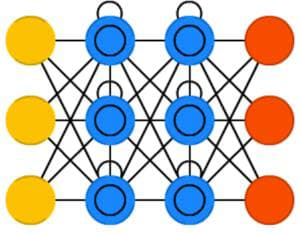
\includegraphics[width=0.75\columnwidth]{./img/recur_2.jpg}
\centering
\caption{Схема строения рекуррентной нейронной сети с долгой краткосрочной памятью}
\label{pic:recur_2}
\end{figure}

Память в LSTM называется ячейками (синие нейроны на рисунке  \ref{pic:recur_2} имеют в себе черный круг, 
символизирующий внутреннюю ячейку памяти). Помимо стандартной для 
рекуррентных нейронов передачи данных - принимают в качестве входных данных 
текущий входной параметр и предыдущее состояние - они имеют специальное внутреннее строение, 
что отличает их от обычной рекуррентной сети. 
Внутри у каждой клетки памяти есть три фильтра: входной, выходной и забывающий, которые решают, какую память сохранить и какую стереть.

\begin{figure}[h]
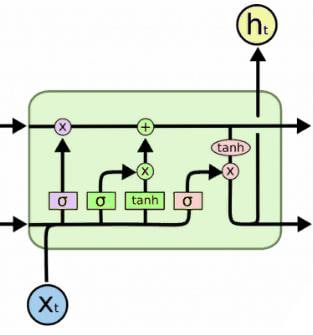
\includegraphics[width=0.75\columnwidth]{./img/recur_3.jpg}
\centering
\caption{Ячейка LSTM в развертке}
\label{pic:recur_3}
\end{figure}

На рисунке \ref{pic:recur_3} изображена ячейка LSTM в развертке. Обозначим 𝑥𝑡 - входное значение (голубой кружок), 
ℎ𝑡 – выходной вектор (желтый кружок). Ячейка состоит из нескольких компонентов, разделенных на три группы по цвету. 
Входной фильтр (компоненты зеленого цвета) определяет, сколько информации из предыдущего слоя будет храниться в клетке. 
Выходной фильтр (компоненты розового цвета) определяет, сколько информации получат следующие слои. 
Ну и забывающий фильтр (компоненты фиолетового цвета) – какую часть информации можно отсечь. 
Целью этих фильтров является защита информации внутри. 
Затем они объединяют предыдущее состояние, текущую память и входной параметр. 

Существуют различные модификации этой «классической» схемы ячейки. 
Сети LSTM способны научиться создавать более сложные структуры, чем классические рекуррентные сети. 
Решение задачи распознавания речи с использованием этой архитектуры было применено в исследовании \cite{2_recur}.

Двунаправленные RNN (Bidirectional Recurrent Neural Networks, BRNN) основаны на той идее, что выход в момент времени t может зависеть не только от предыдущих элементов
15 в последовательности, но и от будущих. Другими словами, сеть будет рассматривать данные как две последовательности – в прямом и в обратном направлении.
Двунаправленные рекуррентные нейронные сети (BRNN) соединяют два скрытых слоя, работающих в противоположных направлениях, 
с одним выходом, позволяя им получать информацию как из прошлых, так и из будущих состояний. 
BRNN разбивает нейроны классической рекуррентной сети на два направления, 
одно для прямых состояний (положительное направление времени), а другое для обратных состояний (отрицательное направление времени). 
Выходы из прямых состояний не связаны со входами обратных состояний, и наоборот. 
Это приводит к общей структуре, которую можно увидеть на рисунке ниже (сеть развернута на 4 временных шага).

Например, если нужно предсказать недостающее слово в середине последовательности (предложения), то нужно учитывать и левый, и правый контекст. 
Двунаправленная рекуррентная нейронная сеть представляет собой две рекуррентные сети, уложенные друг на друга. 
Без обратных состояний эта структура упрощается до обычной однонаправленной прямой RNN. 
Если прямые состояния исключены, получается классическая рекуррентная сеть с перевернутой временной осью.

\begin{figure}[h]
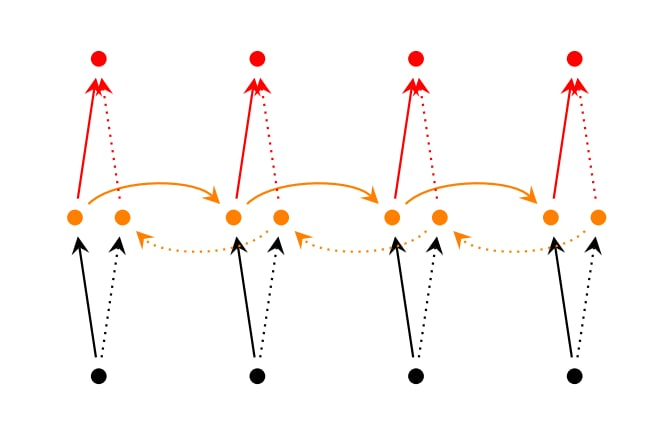
\includegraphics[width=0.75\columnwidth]{./img/recur_5.jpg}
\centering
\caption{Общая структура двунаправленной рекуррентной нейронной сети.}
\label{pic:recur_5}
\end{figure}


На рисунке \ref{pic:recur_5} изображена общая структура двунаправленной рекуррентной нейронной сети (BRNN). 
В процессе её обучения прямые и обратные состояния обрабатываются сначала в прямом проходе 
(на рисунке сплошной линией изображено положительное/прямое направление), выходные нейроны вычисляются последними 
(на рисунке пунктирной линией изображено отрицательное/обратное направление). 
При обратном проходе происходит обратное: сначала обрабатываются выходные нейроны, затем передаются состояния вперед и назад. 
Выход вычисляется на основе скрытого состояния обоих сетей RNN - веса обновляются только после завершения прямого и обратного проходов.

Двунаправленная рекуррентная нейронная сеть находит свое применение в задачи распознавания речи во многих успешных исследованиях \cite{3_recur}.

В последнее время для решения задачи распознавания речи обретает популярность \cite{4_recur}\cite{5_recur}\cite{6_recur} метод, 
использующий свёрточные нейронные сети. Архитектура сети изображена на рисунке \ref{pic:recur_6}.

\begin{figure}[h]
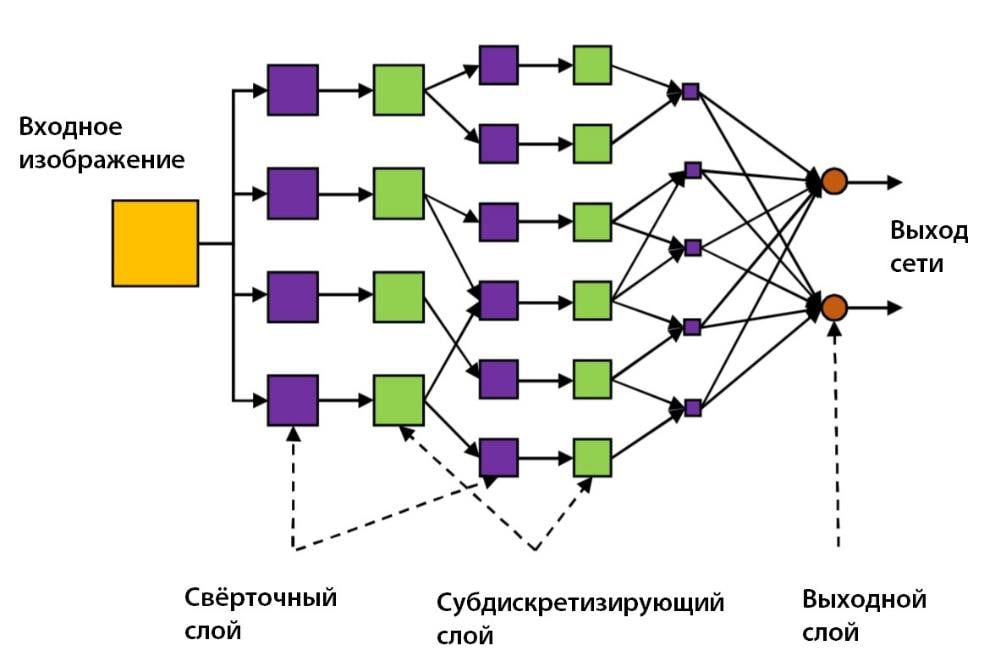
\includegraphics[width=0.75\columnwidth]{./img/recur_6.jpg}
\centering
\caption{Архитектура свёрточной нейронной сети}
\label{pic:recur_6}
\end{figure}

Для описания модели введем обозначения:
\begin{itemize}
  \item $l \in \left[1;L\right]$ - слой нейронной сети, где $L=2n+2$ – количество слоев в сети
  \item $a \in Z^{+}$ - количество скрытых слоёв в сети
  \item $N^l$ - количество карт признаков (фильтров) на слое $l$
  \item $y_n^l$ - $n$-ая карта признаков на слое $l$
\end{itemize}

Карта признаков является тензором и представляет собой выход после каждого слоя сети. 
К примеру, при применении N ядер (свёрток) к одному входному изображению получим N карт признаков. 
Обычно происходит чередование свёрточных и субдискретизирующих (пуллинга) слоёв. 
Тогда свёрточные слои стоят на нечётных позициях $l=1,3,…,2_n+1$, слои субдискретизации на четных позициях $l=2,4,…,2_n$.

Опишем устройство свёрточного слоя. Будем рассматривать слой $l$
, где $l$ принимается нечётный числом $l=1,3,…,2n+1$. Тогда для карты признаков $n$ введем следующие обозначения:

\begin{itemize}
  \item $w_{m,l}^l(i,j)$ – свёртка (ядро, фильтр), применяемая к карте признаков 𝑚 слоя $(l-1)$, на слое $l$ с картой признаков $n$;
  \item $b_n^l$ – пороговые значения, которые присоединяются к карте признаков $n$ на слое $l$;
  \item $V_n^l$ – список всех карт признаков слоя $(l-1)$, которые соединяются с картой признаков $n$ слоя $l$.
\end{itemize}

Таким образом, карта признаков $n$ свёрточного слоя $l$ будет вычисляться следующим образом:

\begin{equation}
  \begin{gathered}
    y_n^l = f_l (\sum_{m \in {V_n^l}} y_m^{l-1} \otimes W_{m,n}^l + b_n^l)
  \end{gathered}
  \label{eq:speach_formula_7}
\end{equation}

Где оператором $\otimes$ обозначена математическая операция двумерной свёртки. Пример вычисления изображен на \ref{pic:recur_7}.

\begin{figure}[h]
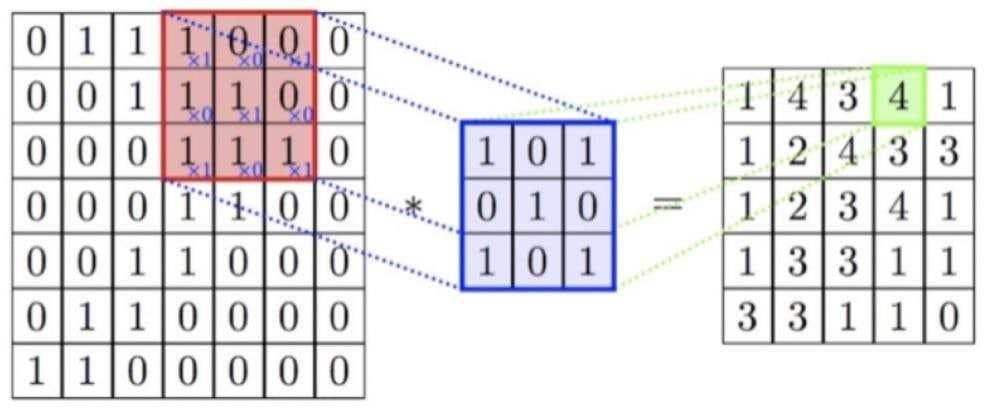
\includegraphics[width=0.75\columnwidth]{./img/recur_7.jpg}
\centering
\caption{Двумерная свёртка карты признаков (слева) и ядра (голубая матрица). \cite{7_recur}}
\label{pic:recur_7}
\end{figure}

Предположим, что размер входных карт признаков $y_m^{l-1}$ равен $H^{l-1} \times W^{l-1}$, 
а размер применяемой к ним свёртки $w_{m,n}^l$ равен $r^l \times c^l$. Тогда размер выходной карты признаков 𝓎𝑚𝑙 вычисляется как:

\begin{equation}
  \begin{gathered}
    (H^{l-1} - r^l + 1) \times (W^{l-1} - c^l + 1)
  \end{gathered}
  \label{eq:speach_formula_8}
\end{equation}

Подробная схема устройства слоя изображена на рисунке \ref{pic:recur_8}. 
Входная карта признаков представлена зеленым квадратом слева, свертка бежевым кругом, 
результат свертки – желтым квадратом. Затем, в случае многомерного фильтра 
(например, в случае работы с многоканальным изображением, когда каждый канал обрабатывается отдельно), 
результаты суммируются по формуле выше и применяется функция активации.
Иначе – желтый квадрат уже является ответом.

\begin{figure}[h]
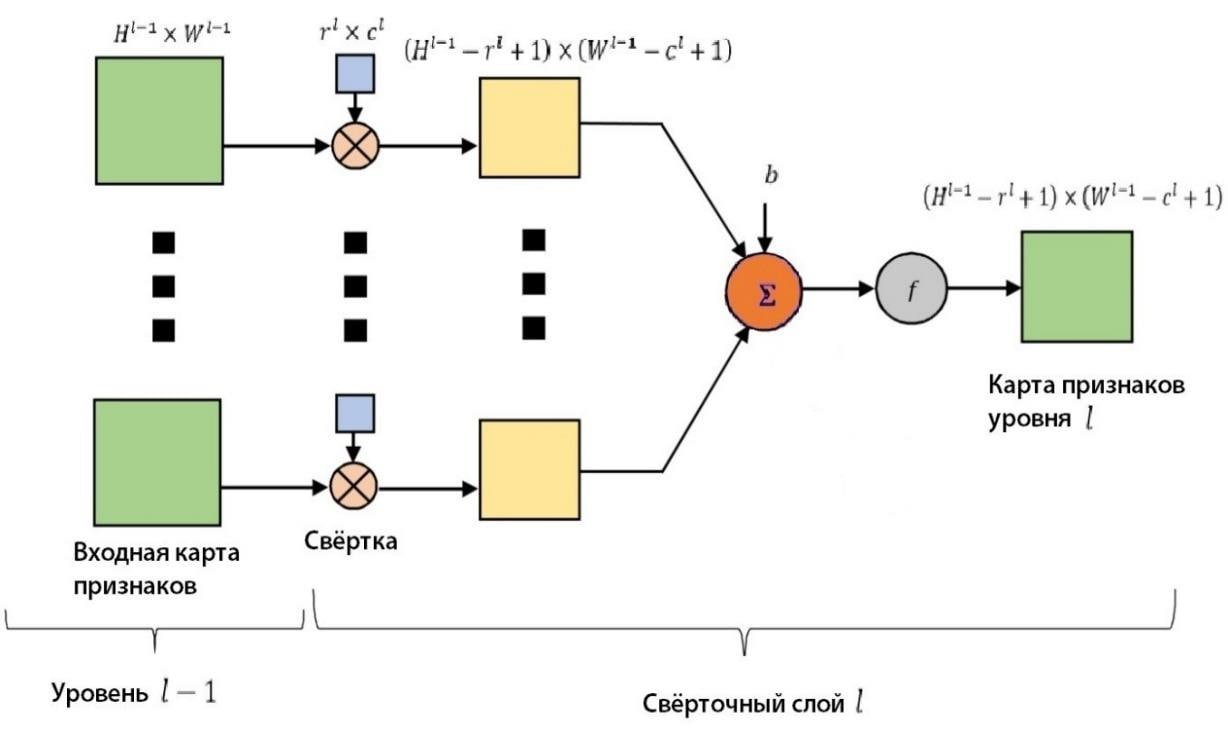
\includegraphics[width=0.75\columnwidth]{./img/recur_8.jpg}
\centering
\caption{Схема свёрточного слоя $l$}
\label{pic:recur_8}
\end{figure}

Введём в рассмотрение субдискретизирующий слой (пуллинговый). Его основная цель – уменьшение размерности входной карты признаков. 
В свёрточной нейронной сети номер $l$ субдискретизирующего слоя принято принимать чётный числом, то есть $l=2,4,…,2a$.

Разделим карту признаков $n (l-1)$ -ого слоя на непересекающиеся блоки размером 2x2 пикселя 
(Для простоты описания используется размер 2x2, однако на практике может использоваться и отличающийся размер). 
Затем просуммируем значения четырёх пикселей в каждом блоке и в результате получим матрицу $z_n^{l-1} = z_n^{l-1} = \left\{ z_n^{l-1}(i,j)\right\}$. 
Её элементами будут являться соответствующие значения сумм. 
Таким образом, формула для вычисления имеет следующий вид:

\begin{equation}
  \begin{gathered}
    z_n^{l-1} = y_n^{l-1}(2i - 1,2j - 1) + y_n^{l-1}(2i - 1,2j) + y_n^{l-1}(2i,2j - 1) + y_n^{l-1}(2i,2j)
  \end{gathered}
  \label{eq:speach_formula_9}
\end{equation}

Картой признаков $n$ субдискретизирующего слоя $l$ будет являться полученная матрица $z_n^{l-1}$. 
При этом вместо суммирования может использоваться любая другая функция (взятие максимума, взятие среднего, суммирование, разность и т.д.). 
Пример вычисления субдискретизирующего слоя с функцией взятия максимума и разбиением на блоки представлен на рисунке \ref{pic:recur_9}.

\begin{figure}[h]
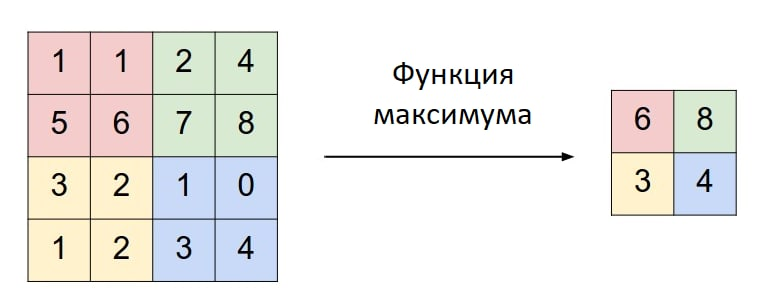
\includegraphics[width=0.75\columnwidth]{./img/recur_9.jpg}
\centering
\caption{Вычисление пуллингового слоя с функцией максимума и блоками 2x2. \cite{8_recur}}
\label{pic:recur_9}
\end{figure}

Таким образом, размер $H^l \times W^l$ карты признаков $y_n^l$ субдискретизирующего слоя $l$ при блоках 2x2 будет равен:

\begin{equation}
  \begin{gathered}
    H^l = \frac {H^{l-1}} {2} \\
    W^l = \frac {W^{l-1}} {2}
  \end{gathered}
  \label{eq:speach_formula_10}
\end{equation}

Существуют модификации слоя субдискретизации. Например, при разбиении карты признаков на блоки, последние могут перекрываться. 
Таким образом, можно задавать шаг смещения следующего блока относительно предыдущего. 
Другая модификация заключается в добавлении дополнительной «пустой рамки» к карте признаков. 
Так, при выполнении операции над блоком, оригинальные (не пустые) ячейки карты признаков могут вносить больший вклад в результат. 
Также, из-за добавления дополнительных ячеек выходная карта признаков будет иметь тот же размер, что и входная.

Выходной слой имеет номер $L=2a+2$, и состоит из $NL$ нейронов. 
Он представляет собой слой обычного многослойного персептрона. Формула для расчета значения выходного нейрона $n$:

\begin{equation}
  \begin{gathered}
    y_n^l = f_l (\sum_{m=1}^{N^{L-1}} y_m^{L-1} \otimes W_{m,n}^L + b_n^L)
  \end{gathered}
  \label{eq:speach_formula_11}
\end{equation}

Где:
\begin{itemize}
  \item $w_{m,n}^L$ – фильтр, применяемый к карте признаков 𝑚 последнего свёрточного слоя для получения перехода к нейрону $n$ выходного слоя (матрица весовых коэффициентов);
  \item $b_n^L$ – пороговое значение, добавляемое к нейрону $n$ (коэффициент сдвига).
\end{itemize}

Таким образом, выходом свёрточной нейронной сети является вектор следующего вида:

\begin{equation}
  \begin{gathered}
    y = \left[ y_1^L,y_1^L, ...,  y_{N^L}^L\right]
  \end{gathered}
  \label{eq:speach_formula_12}
\end{equation}

Для применения свёрточных сетей в задаче распознавания речи первоначально используется спектральное представление звукового потока.

\begin{figure}[h]
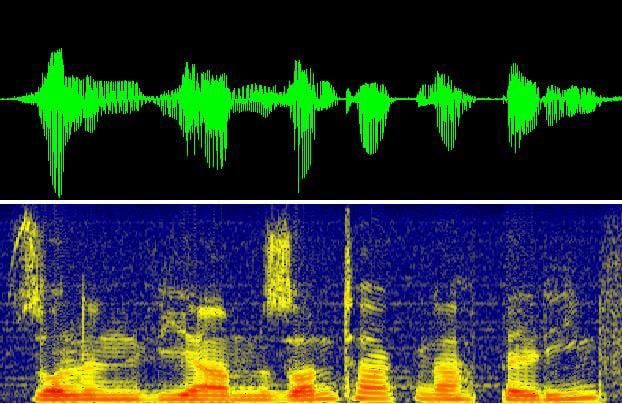
\includegraphics[width=0.75\columnwidth]{./img/recur_10.jpg}
\centering
\caption{ Изображение звуковой дорожки и соответствующего ей спектрального представления. Источник \cite{9_recur}}
\label{pic:recur_10}
\end{figure}

На основе полученного спектрального изображения (на рисунке \ref{pic:recur_10} изображена звуковая дорожка и соответствующее ей спектральное представление) 
стандартная свёрточная сеть для обработки спектрального представления сигнала выдает готовый распознанный результат.

\section{Семантический анализ текста и его виды}

Помимо анализа текста посредством опредения тональности текста, одним из типов анализа текста - является
семантический анализ текстов.

% тут надо нормально проставить cit
Семантический анализ текста – одна из основных проблем как 
теории создания систем искусственного интеллекта, относящаяся 
к обработке естественного языка (Natural Language Processing, NLP), так
и компьютерной лингвистики. В наш век компьютерных технологий
чрезвычайно важно получать информацию на естественном языке и
сделать так, чтобы эта информация могла перерабатываться с помощью
компьютера [4: 208]. 

На текущий момент выделяют следущие модели семантического анализа текста:
\begin{enumerate}
  \item Семантическая сеть
  \item Фреймовые модели
  \item Онтологическая модель
  \item Тезаурус 
\end{enumerate}

Семантическая сеть – модель предметной области, имеющая вид
ориентированного графа, вершины которого соответствуют объектам
предметной области, а дуги (ребра) задают отношения между ними.
Семантическая сеть появилась на основе математических формул. Семантическая сеть представляет собой схему, где есть концепты предметов, событий, состояний, с помощью линий показано отношение между
концептами.


Фреймовые модели – это структура, которая нужна для того, чтобы
описать понятия или ситуации, состоящая из характеристик этой ситуации и их значений. Фрейм можно считать элементом семантической
сети.

Онтологическая модель – это детальное описание какой-то предметной или проблемной области, которое можно использовать для
формулирования утверждений общего характера. Эта модель помогает
создавать понятия, которые впоследствии становятся пригодны для машинной обработки.

Тезаурус – лексический словарь, в котором показаны семантические отношения между лексическими единицами.
Благодаря этому словарю можно понять смысл, не только с помощью определения, но и соотнеся слова с другими понятиями и их группами, 
благодаря чему можно использовать искусственный интеллект для того, чтобы наполнить базы знаний. 
Обычно в тезаурусах используют такие семантические
отношения как, синонимы, антонимы, гипонимы, гиперонимы, меронимы, холонимы и паронимы. 
WordNet можно привести как пример тезауруса. 
Синсет (синонимический ряд) является основной словарной единицей WordNet, 
он объединяет слова с похожими значениями. Синсеты
это слова одной и той же части речи, что и слово, которое вы вводите. У
каждого такого слова есть своя дефиниция, которая объясняет значение
этого слова. Например, к слову ручка (pen) в таком словаре есть разные
значения: crayon, pencil, marker.

Из вышеперечисленного можно сделать вывод, что в век компьютеризации, 
вопрос о семантическом анализе текста становится все более
популярным. Из-за этого, область автоматической обработки текстов
сфокусировалась на прикладном аспекте. Семантический анализ представляет 
собой одну из сложных математических задач, несмотря на
востребованность практически во всех областях жизни современного
человека. Главной задачей является сделать так, чтобы компьютер смог
корректно трактовать образы, которые авторы текстов хотят передать
читателям или слушателям. 

%акустика
\section{Wav2vec}
Текущие современные модели распознавания речи требуют больших объемов расшифрованного звука.
Данные для достижения хороших результатов. В последнее время предобучение нейронных сетей
стал эффективным методом для условий, где размеченных данных недостаточно. Ключевая идея состоит в том, чтобы
изучить общие представления в установке, где имеется значительное количество размеченных или неразмеченных данных.
Доступны и использовать изученные представления для повышения производительности в последующей задаче.
для которых количество данных ограничено. Это особенно интересно для задач, где существенные
требуются усилия для получения помеченных данных, таких как распознавание речи.

В данный момент принято использовать предварительное обучение для для улучшения распознавания речи с учителем. Это
позволяет использовать немаркированные аудиоданные, которые гораздо проще собрать, чем помеченные данные.
Под предварительным обучением подразумевается факт обучения нейронной сети для задачи, в которой исользуется.
большой объем данных. 
Это широко применялось в "computer vision", обработке естественного языка и, в последнее время, для определенных речевых задач.

Предварительное обучение бывает: 

\begin{itemize}
  \item контролируемым образом
  \item в неконтролируемом режиме
\end{itemize}

Предварительное обучение похожа на трансферное обучение, когда вы предварительно обучаете модель, зная что есть $X$ и $y$.
Но для неконтролируемого предварительного обучения вы изучаете представление речи. 
wav2vec — это сверточная нейронная сеть (CNN), которая принимает необработанный звук 
в качестве входных данных и вычисляет общее представление, 
которое может быть введено в систему распознавания речи. 
Целью является контрастная потеря, которая требует отличить истинный будущий звуковой образец от негативов.

Учитывая контекст входного сигнала цель состоит в том, чтобы предсказать следующую обсервацию из этого образца речи.
Есть сопутствующая проблема, которая заключается в том, что следует иметь четкое представление как именно 
моделировать распределение $p(x)$ для речевых примеров. Решение это проблемы заключается в том что 
следует понизить размерность образцов речи при помощи "сети кодировщика", а уже затем использовать
контекстную сеть для прогнозирования следующих значений. 
wav2vec изучает представления аудиоданных, решая задачу прогнозирования контекста.

Конкретно




\section{SVC}
\section{kNN}
\section{MLP}


\section{Выводы}

% В данном разделе была сформулирована постановка задачи, рассмотрены возможные ее решения с помощью архитектуры eBICA и подхода с использованием машинного обучения. 
% Выделен подход для распозвавания речи.

Было изучено описание работы модели виртуального актора. Изучены подходы и методы применительно к задаче распознавания речи.
Были рассмотрены ключевые подходы машинного обучения, которые будут использоваться в работе, а именно рекуррентные нейронные сети


\clearpage

\chapter{Проектирование модели поведения виртуального агента}

В этом разделе описывается и обосновывается выбор инструментария для проектирования и программного воплощения 
модели поведения актора в заданной парадигме. Описываются ключевые моменты проектирования и программной реализации модели поведения актора.

\section{Описание предыдущей модели поведения актора и виртуального окружения}

В ходе выполнения программы записывались данные с оценками для первого и второго клоуна, а также с выводом сообщения совершенного 
действия, данные представлены на (Рис. \ref{pic:ris10}).

\begin{figure}[h]
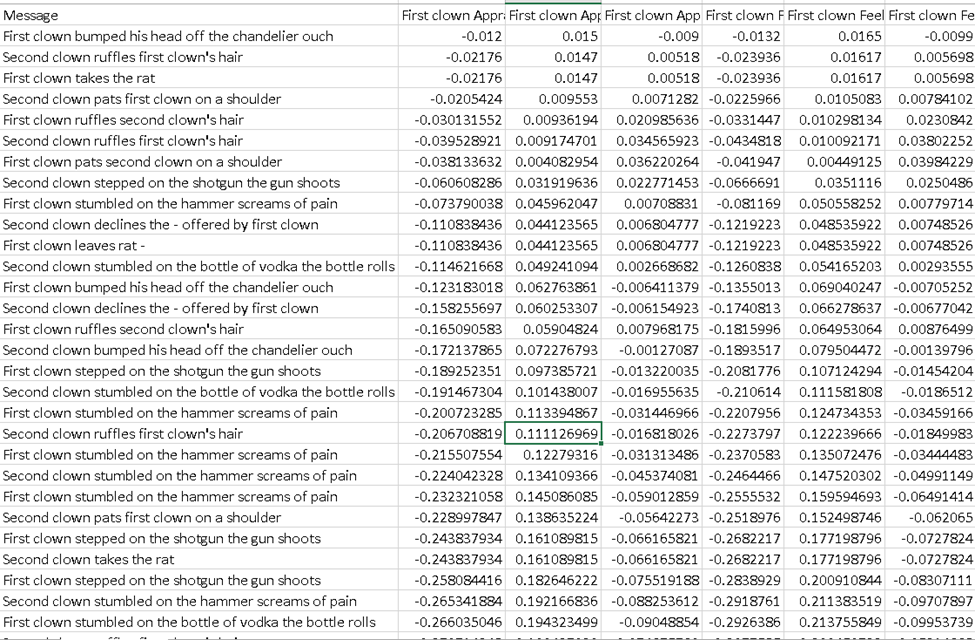
\includegraphics[width=0.75\columnwidth]{./img/ris10.png}
\centering
\caption{Оценки и действия совершенные первым виртуальным актором}
\label{pic:ris10}
\end{figure}

Для осуществления контроля за действиями акторов и их анализом система ведет записи в журнал событий. 
Журнал представляет собой текстовую таблицу. Записи выглядят следующим образом: каждая строка журнала соответствует своему событию, 
строка начинается с указания времени, когда была произведена запись. После указания времени указывается тип сообщения. 
Далее в сообщении показывается исполнитель действия, цель действия и номер действия из таблицы действий. 
После идет содержание сообщения, поясняющее произошедшее событие. После чего показаны оценки Appraisals и 
Feelings для доброжелательности, возбужденности и доминантности.

На (Рис. \ref{pic:ris11}) представлены гистограммы частот действий, совершаемых испытуемыми и модельным человеком.

\begin{figure}[h]
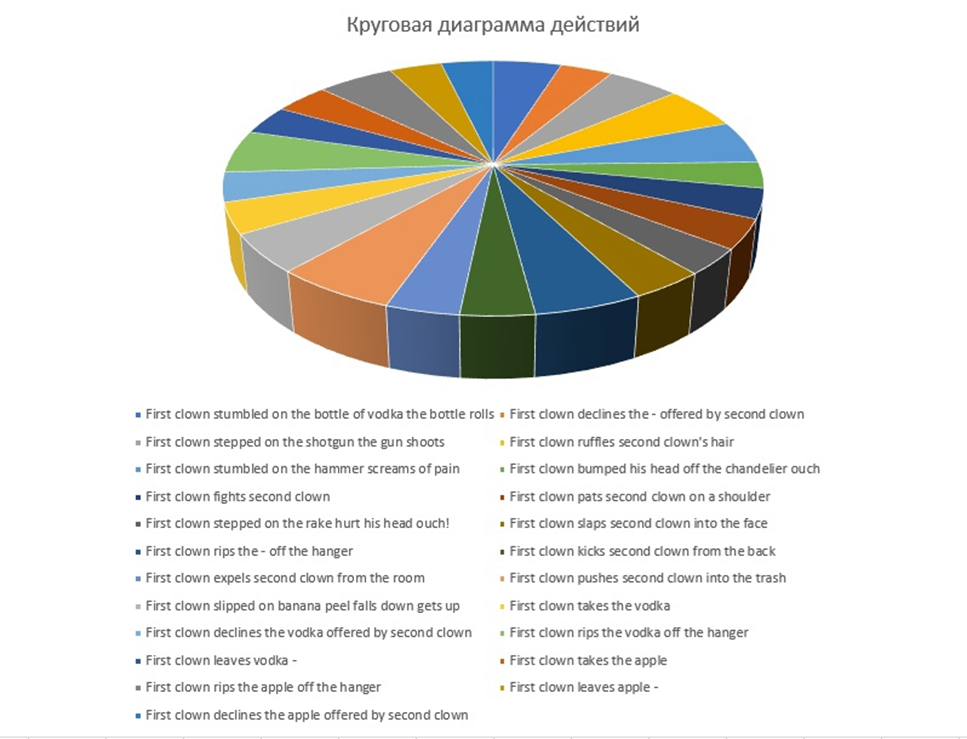
\includegraphics[width=0.75\columnwidth]{./img/ris11.png}
\centering
\caption{Диаграмма частот действий первого актора}
\label{pic:ris11}
\end{figure}

Исходя из диаграммы, можно заметить, что большое количество действий не использовалось. 
Данная ситуация возникла в ходе тестирования взаимодействия роботов с использованием моральной схемы, описанной в формуле \ref{eq:appraisals01}.

Существенным фактором, повлиявшим на работу моральной схемы, является оценка каждого действия отдельно по VAD, о чем говорися в работе \cite{Samsonovich02}. 
В ходе корректировки действий, основанной на опросе фокус группы, были произведены корректировки оценок. 
Результат корректировок виден на (Рис. \ref{pic:ris11}).

\section{Сбор данных, метрики и инструменты}

Для реализации сбора информации обычно используются следующие инструменты,  что отображено в работае \cite{parser01} :
\begin{itemize}
  \item	HTTP Client – клиент является библиотекой передачи, он находится на стороне клиента, отправляет и получает сообщения HTTP.
  \item	Beautiful Soup - это пакет Python для анализа документов HTML и XML. Он создает дерево синтаксического анализа для проанализированных страниц, которое можно использовать для извлечения данных из HTML, что полезно для парсинга веб-страниц.
  \item	Requests - это HTTP-библиотека для языка программирования Python. Цель проекта - сделать HTTP-запросы более простыми и удобными для человека.
  \item	AsyncIO – модуль, предназначенный для упрощения использования корутин и футур в асинхронном коде — чтобы код выглядел как синхронный, без коллбэков.
\end{itemize}

Основной принцип парсинга ресурсов для сбора информации осуществлялся при помощи написания алгоритмов на языке программирования Python. Для этого использовалась библиотека ButifulSoup, которая была выбрана для использования для чтения HTML, а также библиотека Requests, которая является стандартным инструментом для составления HTTP-запросов в Python. Простой и аккуратный API значительно облегчает трудоемкий процесс создания запросов. Таким образом, можно сосредоточиться на взаимодействии со службами и использовании данных в приложении. Так же из за большого количества реквестов было рационально использовать корутину, используя библиотеку Asyncio.

Такие HTTP методы, как GET и POST, определяют, какие действия будут выполнены при создании HTTP запроса. 
GET является одним из самых популярных HTTP методов. Метод GET указывает на то, что происходит попытка извлечь 
данные из определенного ресурса. Для того, чтобы выполнить запрос GET, используется requests.get(). 
Положительным ответом сервера является код 200. 

В метод requests.get() помещается URL, в которую может быть помещен JSON как текст запроса, либо при наличии 
API более упрощенный текстовый параметр, при наличии  токена как идентификатора аккаунта – токен.

response.status\_code, который равен 200, означает то что ответ от сервера получен положительный, 
текст запроса обработка, идентификация пользователя прошла успешна, возвращен ответ в формате JSON.

Иной же случай, когда нет доступа к API, оно платное либо его не существует. 
В таком случае скрипт будет выглядеть следующим образом.

В данном примере осуществляется request по URL, добавляется User-Agent, который имитирует пользователя, 
декодируются данные HTML в формат Unicode-8, который представляет собой распространённый стандарт 
кодирования символов, позволяющий более компактно хранить и передавать символы Юникода, используя 
переменное количество байт, и обеспечивающий полную обратную совместимость с 7-битной кодировкой ASCII.

Далее находим все классы таблиц и присваиваем переменным генератор, вытаскивающий 
из классов таблиц данные с соответствующим тегом.

С помощью BS4 можно найти в коде HTML все что требуется для создания нудного массива данных, 
далее для того, чтобы унифицировано хранить данные, следует использовать объектно-ориентированные форматы 
данных, такими бывают JSON и XML. JSON - текстовый формат обмена данными, основанный на JavaScript. 
Как и многие другие текстовые форматы, JSON легко читается людьми и в итоге был выбран как формат хранения данных в работе.

Для того чтобы спарсить сайт полностью и извлечь весь требуемый тип данных, используются рекурсивный подход. 
Для этого в работе используется пакет Python - html5lib, который реализует алгоритм парсинга HTML5, 
на который сильно влияют современные браузеры. Как только парсер получает нормализованную структуру 
содержимого, становится доступным поиск данных в любом дочернем элементе тега html. 
Искомые данные чаще всего находятся в теге “table”. После нахождения родительского тега, рекурсивно проходим по дочерним элементам. 
Для ссылок чаще всего используется тег “href”, далее из полученных ссылок извлекаем требуемый тип данных на сайте, в нашем случае это текст. 

Так как на сайте слишком много текста и достаточно большой процент содержания лишнего текста по типу маркировок, 
контекстной рекламы и прочего, ставится задача определения выявления значимого текста на сайте. 

Значимый текст выбирается на основании анализа его принадлежности к заранее определенным классам текста (или тематикам). 
Как правило, методы автоматической классификации основаны на методе машинного обучения: сначала получают 
обученную с помощью какого-либо алгоритма модель, качество которой определяет точность классификации. 
Таким образом, процесс обучения зависит от выбранного алгоритма и «чистоты» обучающей выборки, согласно работе о \cite{neural04}. 
Одним из фреймворков, который используется для того чтобы обучать модель по заранее определенным классам – это lingvo, 
реализованный для  .NET Framework, в котором используется Gradient Sign Dropout (GradDrop).

\section{Инструменты для анализа текста}

После сбора данных для их последующего использования в нейронной сети требуется осуществить разметку данных, для этого требуется 
выделить те слова определяющие какое-либо действие или предмет, которые будут семантически близки к заранее предопределенным 
типам действий или типам предметов.

Возможность идентификации семантической близости между словами сделала модель word2vec широко используемой в NLP-задачах, которые подробно описываются в \cite{neural05}. 
Идея word2vec основана на контекстной близости слов. Каждое слово может быть представлено в виде вектора, 
близкие координаты векторов могут быть интерпретированы как близкие по смыслу слова \cite{seman04}. 

Таким образом, извлечение семантических отношений (отношение синонимии, родовидовые отношения и другие) может быть автоматизировано. 
Установление семантических отношений вручную считается трудоемкой и необъективной задачей, требующей большого количества времени и 
привлечения экспертов. Но среди ассоциативных слов, сформированных с использованием модели word2vec, встречаются слова, не 
представляющие никаких отношений с главным словом, для которого был представлен ассоциативный ряд \cite{seman03}.

В работе рассматриваются дополнительные критерии, которые могут быть применимы для решения данной проблемы. Наблюдения и проведенные 
эксперименты с общеизвестными характеристиками, такими как частота слов, позиция в ассоциативном ряду, могут быть использованы для 
улучшения результатов при работе с векторным представлением слов в части определения семантических отношений для русского языка. 

Представление слов в виде векторов позволяет применять математические операции. В большинстве примеров можно встретить вычитание векторов, 
когда результат вычисления vec('Madrid') - vec('Spain') + vec('France') будет ближе к vec('Paris'), чем к другим векторам из распределения. 
Таким образом, разница векторов может быть использована для поиска семантических отношений между словами \cite{seman02}.

Word2vec не возвращает напрямую семантические отношения между словами. В ассоциативном ряду, который может быть возвращен 
в качестве близких слов к запрашиваемому (главному) слову, отражаются слова, которые часто употребляются рядом в контексте. 
Бесспорно, в ассоциативном ряду встречаются синонимы, антонимы, гипонимы, гиперонимы, холонимы, меронимы, ассоциации и другие 
типы, которые могут быть определены как семантические отношения.

\section{Диаграмма классов}

На (Рис. \ref{pic:ris12}) изображена диаграмма классов (Построение такой диаграммы рекомендуется в работе \cite{OOP}):

\begin{figure}[h]
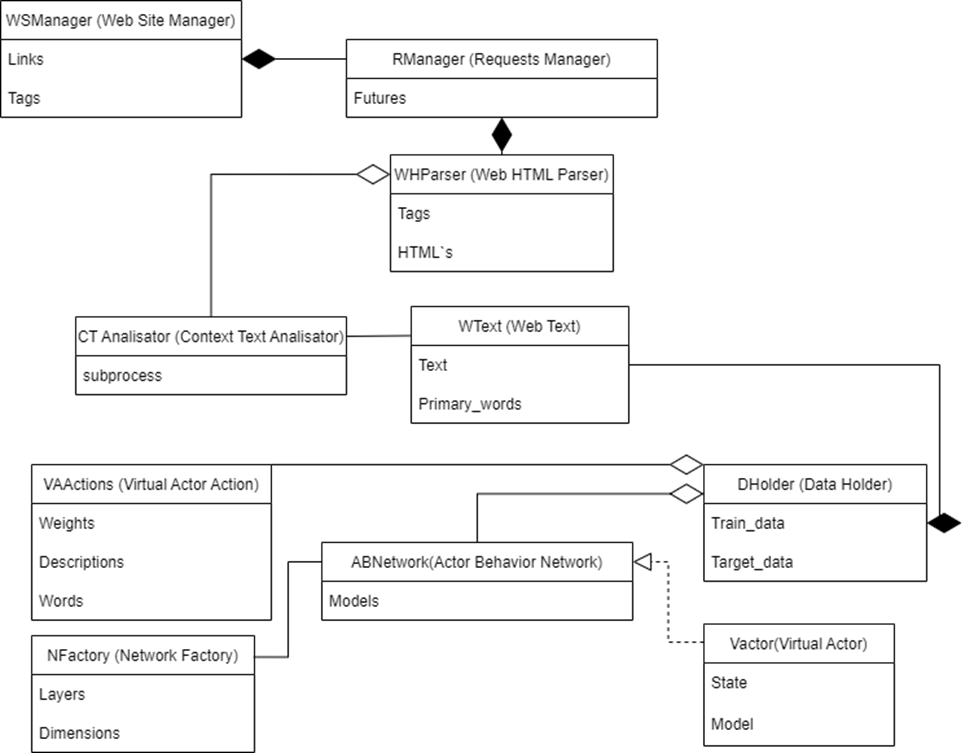
\includegraphics[width=0.75\columnwidth]{./img/ris12.png}
\centering
\caption{Связь между акторами и объектами}
\label{pic:ris12}
\end{figure}

\begin{enumerate}
  \item	В Web Site Manager попадают ссылки на все сайты, каждому сайту указываются теги.
  \item	Далее Web Site Manager передает ссылки в Request Manager.
  \item	Request Manager асинхронно посылает запросы на сайт, чтобы получить весь контент сайта, по запросу он получает html-страницу и передает ее в Web Html Parser.
  \item	Web Html Parser по тегам парсит html так, что выделяет нужный текст, который передается в Web Text.
  \item	Context Text Analisator -  использует консольное приложение по работе с LingvoNET, с которым класс общается посредством стандартного ввода/вывода с целью классификации текста на предмет семантической принадлежности.
  \item	В Web Text выделяются ключевые слова при помощи Virtual Actor Action.
  \item	Virtual Actor Action берутся из excel-таблицы действий со значением весов и описаниями.
  \item	В Data Holder на основании Virtual Actor Action и самого текста генерируются сценарии (10 действий, 11 состояний), моделью пытаемся предсказать 11 состояние на основе 10 предыдущих.
  \item	Actor Behavior Network хранит все обученные модели, из которых потом выбирается оптимальная.
  \item	Network Factory – шаблон проектирования, создает по описанию нейронной сети создает экземпляр сети (Actor Behavior Network).
  \item	Одному Virtual Actor соответствует одна нейронная сеть, у Virtual Actor меняется текущее состояние на основе модели. 
\end{enumerate}

\section{Выводы}

В процессе работы были выделены часто используемые инструменты для сбора данных со сторонних веб-сервисов, 
а именно программные модули языка Python requests, Asyncio, ButifulSoup. 
Произведен анализ инструментария для решения задач семантической близости слов. 
Также была составлена диаграмма классов программного модуля. 
А для моделирования поведения виртуального агента составлена архитектура рекуррентной нейронной сети.





\clearpage

\chapter{Реализация программного продукта}

В данном разделе приводятся измененный алгоритм поведения Виртуального Актора.

\section{Текущая версия реализованной модели}

Для решения задачи разработки экспериментальной платформы на базе виртуального окружения для изучения социально – эмоционального поведения 
акторов целесообразно использовать специальные программные окружения для разработки виртуальных окружений и сопутствующих компонент – «игровые движки». 
По результатам анализа стало понятно, что такая среда должна прежде всего обладать:

\begin{enumerate}
  \item Большим сообществом разработчиков
  \item Подробной документацией
  \item Относительно низкой сложностью
  \item Простотой установки
  \item Модульной системой
\end{enumerate}

Всеми данными свойствами обладает лишь Unity3D, как самый распространённый, на данный момент инструмент построения виртуальных окружений. 
На базе Unity3D сделано больше игр, чем на любой другой технологии, поэтому он и обладает наиболее развитым сообществом разработчиков на данный момент. 
В сети имеется большое множество документации и курсов по данной технологии. Благодаря модульной системе, можно найти специальные программные модули, 
которые легко встраиваются в разработанный продукт, расширяя возможности всей системы.  Преимуществом данной среды также следует считать относительную 
простоту переноса разработанного виртуального окружения на другие платформы (например, смартфоны, планшеты или же любую из существующих операционных систем). 
Также стоит отметить, что программная среда имеет бесплатную лицензионную версию для небольших команд разработчиков.

Unity предлагает разработчику возможность использовать три различных сценарных языка: C\#, JavaScript (его модификация) и Boo (собственный диалект Python). 
Для разработки данной экспериментальной платформы был выбран C\#, как де факто, стандарт при разработке на Unity3D. 

В качестве среды разработки используется Visual Studio 2019. Для контроля версий использовать облачное хранилище Dropbox и GitLab. 
В качестве средства проектирования использовался стандартный модуль Visual Studio для построения диаграмм классов.

\begin{figure}[h]
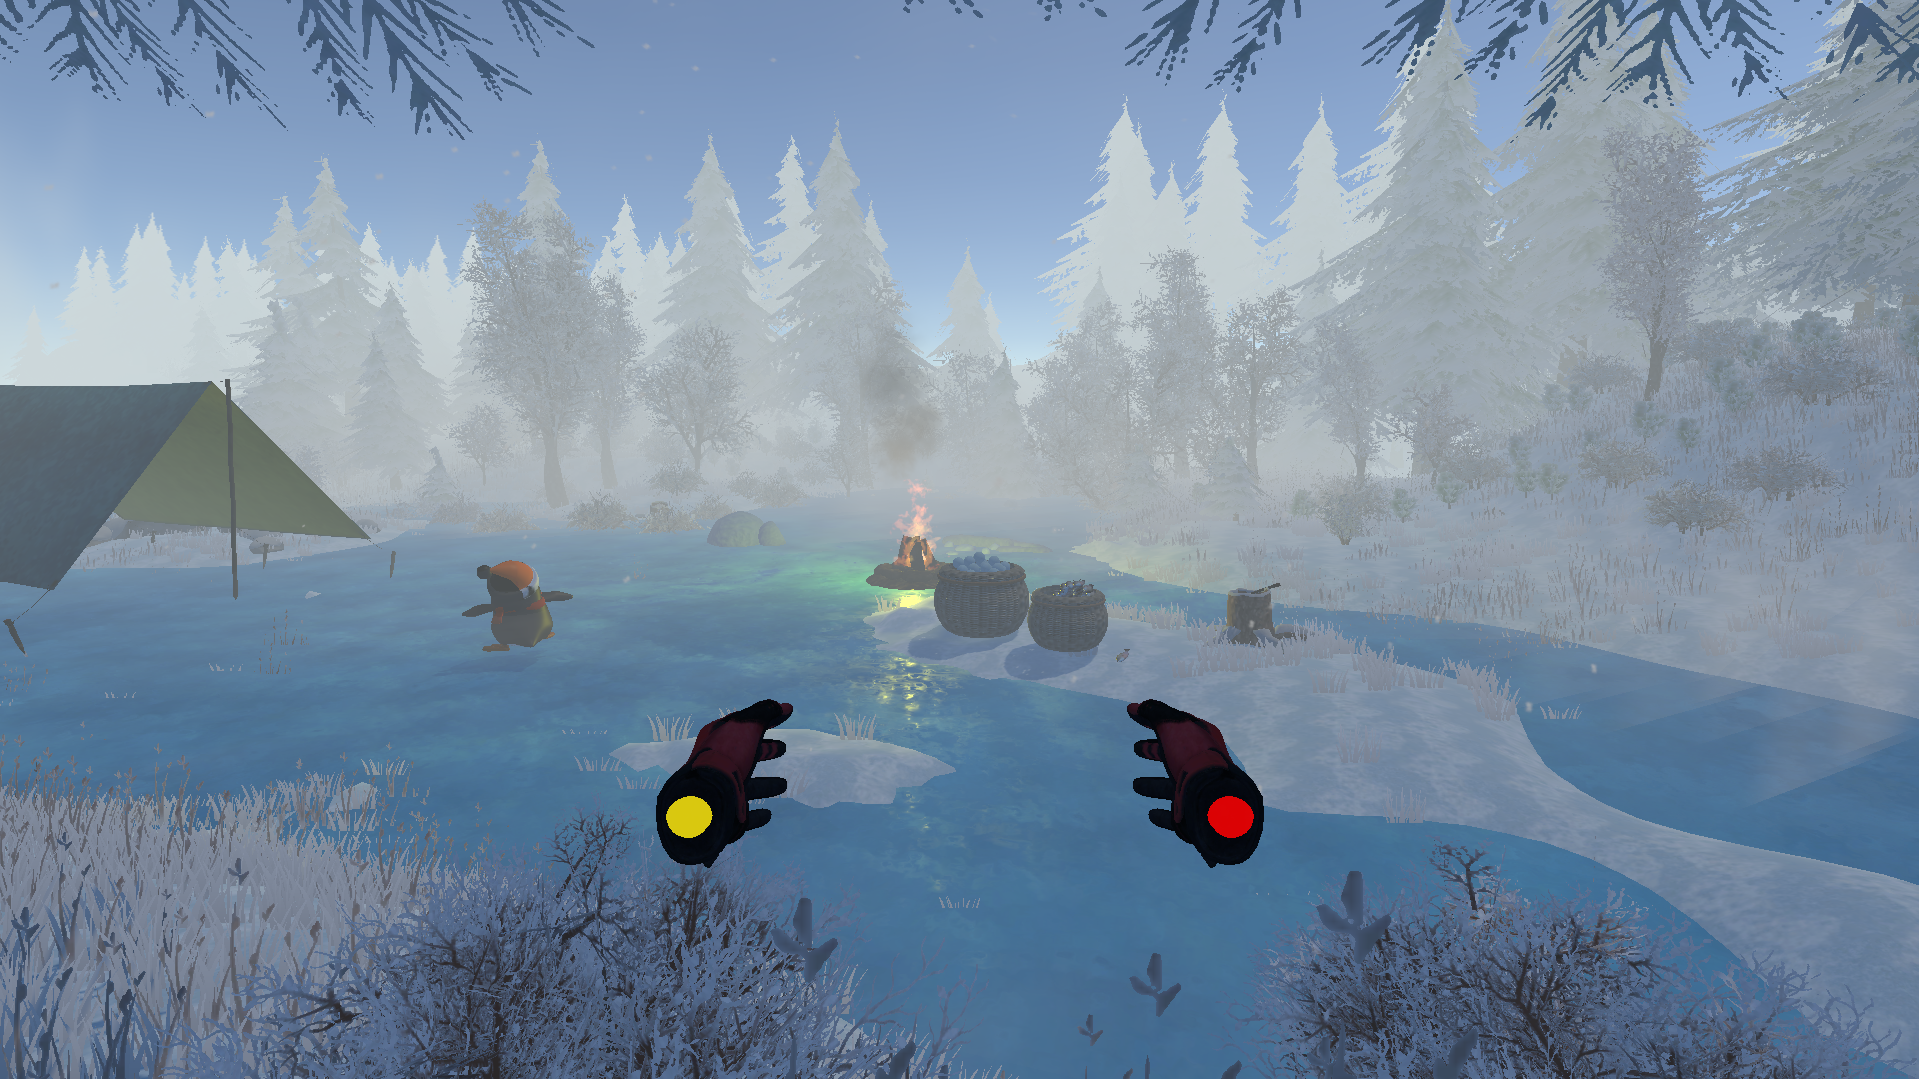
\includegraphics[width=0.75\columnwidth]{./img/penis.png}
\centering
\caption{Cкриншот взаимодействия человека с Виртуальным Актором}
\label{pic:penis}
\end{figure}

В работе было реализовано программное приложени с помощью движка юнити результаты работы которого вы можете видеть на (рис. \ref{pic:penis})

\section{Интеграция моделей из python в C\#}

В расширенной диаграмме классов, было выделено какие стадии обработки проходит аудио-запись (Рис. \ref{pic:ncmodel0}).

Получение Audio из UNITY3D осуществлялось при помощи ксласса Microphone и далее помещалось 
в контейнер для аудио данных AudioClip, который хранит аудиофайл либо сжатым в ogg vorbis, либо без сжатия.

Далее, полученная аудио проходит обработку при помощи моделей реализовнных на языке программирования python, 
при непосредственном использовании IronPython, который представляет из себя реализацию языка программирования 
Python с открытым исходным кодом, которая тесно интегрирована с .NET Framework. 
IronPython может использовать библиотеки .NET Framework и Python, а другие языки .NET могут также легко использовать код Python».

Мы использовали метод ExecuteFile(), так как в нашем случае он самый подходящий.

В указанном выше методе проиходит следующее:
\begin{itemize}
  \item В коде C\# в метод ExecuteFile(@"/home/...") помещен путь к файлу .py
  \item Функция из Python определяется в C\#,
  \item Возвращается результат по заврешнию исполнения кода .py,
\end{itemize}

Таким образом проиходит интеграция реализации динамического языка программирования IronPython в проект.

\section{Команды испольняемые посредством распозавания речи}

Процесс распозавнания речи проводился частично посредством использования 
внутренного инструментария UNITY3D. В нем пакет HoloToolKit Unity
предоставляет несколько методов голосового ввода. В нашем случае был 
выбран метод DictationRecognize который обладает функцией преобразования 
текста в речь. 

Для того чтобы пользователь мог передавать голосовые фразы приложению, следует:

\begin{itemize}
  \item Создать объект DictationRecognize
  \item Произвести инициализацию процесса диктовки
\end{itemize}

Однако HoloToolKit Unity не дает возможности распознавать речь на
русском языке, в связи с чем был использован лишь для сохранения 
аудио в формате ".wav". Сама процедура распознавания речи прводится
с помощью YandexSpeechKit. Для этого был получен уникальный 
IAM-токен для возможности использовать API. Реализовано простое приложение, 
которое получает распознанную речь в формате JSON 

Пример запроса: 

\lstinputlisting[
  float=ht,frame=lines,label=lst:queryjson,caption=Пример запроса
]
{listings/query.json}

Пример ответа: 

\lstinputlisting[
  float=ht,frame=lines,label=lst:queryjson,caption=Пример ответа
]
{listings/answer.json}

Далее посредством определения семантической близости слов по распознанной речи 
выявляются команды для Виртуального Питомца. Полученная последовательность 
команд передается в ActionsAlgothms, где производится временное изменение 
вероятностей выполнения действий. Данные изменения действуют до выполнения 
любого действия, а после сбрасываются. Действие соотносящееся с командной 
повышают свою вероятность исполнения, тогда как остальные понижают. Если 
Действие для которого была передана команда из последовательности командне будет 
выполнена, то остальная часть последовательности не будет провоцировать изменение
в классе ActionsAlgothms. 

Стек возможных команд представлен ниже:

\begin{itemize}
  \item Играть в снежки с человеком 
  \item Играть в снежки с испытуемым
  \item Пищать
  \item Подойти к человеку
  \item Подойти к испытуемому
  \item Пойти спать
  \item Посмотреть в сторону человека
  \item Посмотреть в сторону испытуемого
  \item Поприветствовать человека
  \item Поприветствовать испытуемого
  \item Подойти к корзине с рыбой и поесть
  \item Поесть из рук
\end{itemize}




\section{Реализация и дообучение модели}

Как говорилось ранее для создания возможности эмоционального взаимодействия пользователя с виртуальным актором - 
берется предобученная модель "jonatasgrosman/wav2vec2-large-xlsr-53-russian". Данная модель 
работает в состве библеотки huggingsound. На выходе модели для отдельного аудиофайла получаются 512-мерные вектора. 
Далее высчитывается средней вектор, который передается в модели для распознования эмоций.
Используется python3.8 и библиотека машинного обучения pytorch и sklearn.

Для SVC с ядром RBF менялся параметр регурялизации, а именно он принимал значения 1, 10 и 100.

Для k-NN менялось количество соседей от 10 до 40 с шагом в 10.

Для MLP выходной слой не менялся и состоял из 8 нейронов, тогда как количество внутрених слоев менялось от 1 до 3 так,
что количество нейронов в них оставалось неизменным и равным 1024.
В качестве функции активации была выбрана функция гиперболического тангенса.

Были выделены следющие эмоции для распознавания акустическим методом из речи:

\begin{enumerate}
  \item Злость
  \item Спокойствие
  \item Отвращение
  \item Ужас
  \item Счастье
  \item Нейтральность
  \item Грусть
  \item Удивление
\end{enumerate}

В результате чего был получен следующий результат (таб. \ref{pic:table}): 

\begin{figure}[h]
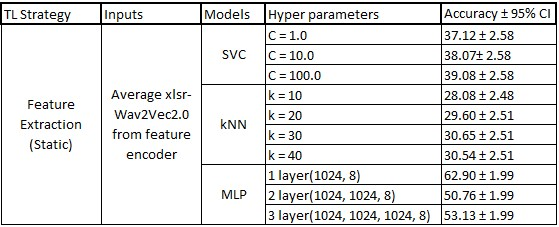
\includegraphics[width=0.75\columnwidth]{./img/table_all_em.jpg}
\centering
\caption{Результаты обучения по 8 выделенным эмоциям}
\label{pic:table}
\end{figure}

Однако результат был не удовлетворительным в связи с чем было принято решение 
упростить классфикацию эмоций на положительные и отрицательные следущим образом (таб. \ref{tbl:em_table}):

\begin{table}[H]
\caption{Разделение эмоций по классам с оценкой}
\label{tbl:text_a00}
\begin{center}
%\centering

\begin{tabular}{ | c | c | c | }
  \hline
  Злость & Отрицательные & -1 \\ \hline 
  Спокойствие & Пололожительные & 1 \\ \hline 
  Овращение & Отрицательные & -1 \\ \hline 
  Ужас & Отрицательные & -1 \\ \hline 
  Счастье & Пололожительные & 1 \\ \hline 
  Нейтральность & Пололожительные & 1 \\ \hline 
  Грусть & Отрицательные & -1 \\ \hline 
  Удивление & Пололожительные & 1 \\ \hline 
\end{tabular}
\end{center}
\end{table}

В соответствии с новым подходом соответствия эмоции одному из двух классов, а именно 
положительному или отрицательному, было получен следующий результат показанный на таблице \ref{pic:table2}:

\begin{figure}[h]
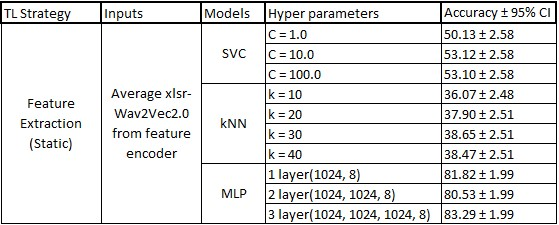
\includegraphics[width=0.75\columnwidth]{./img/table_2_em.jpg}
\centering
\caption{Результаты обучения по классификации эмоций на положительные и отрицательные}
\label{pic:table2}
\end{figure}

В результате чего был получен удовлетврорительный результат.
При обучении датасет разбился на парти в 100 образцов в каждой так, чтобы была возмножность
обучать модели на GPU. Обучение проводилось до 10 эпох так, что результирующей модеью становилась та,
что показывала максимальный результат в какой-либо эпохе.
Так как ставится задача классификации, то в качестве функции потерь используется функция потерь перекрестной энтропии.
В качестве опитимизатора использовался оптимизатор Адам.


\section{Результаты}

В результате было получено следующее взаимодействие, представленное на рисунке \ref{pic:res_actions_plus_voice_actions}:

\begin{figure}[h]
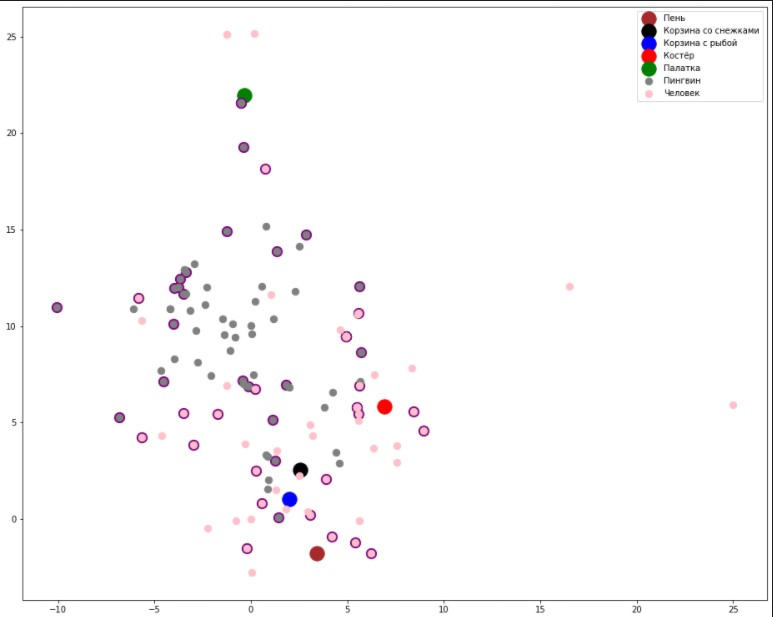
\includegraphics[width=0.75\columnwidth]{./img/res_actions_plus_voice_actions.jpg}
\centering
\caption{Карта перемещений Виртуального Актора и человека}
\label{pic:res_actions_plus_voice_actions}
\end{figure}

Условные обозначения: 

\begin{itemize}
  \item Синий кружок - Корзина с рыбой
  \item Коричневый кружок - Пень
  \item Черный кружок - Корзина со снежками
  \item Красный кружок - Костер
  \item Зеленый кружок - Палатка
  \item Серый кружок - Пингвин
  \item Розовый кружок - Человек
  \item Выделенный кружук фиолетовым - отклик одного из акторов на команду
\end{itemize}

Рисунок предоставляет собой карту где точки находятся на виртуальной сцене 
серым и розовым отмечаются где происходило взаимодейтвия акторов, эти 
места с фиолетовым ободком обозначают, что взаимодейтвие было инициировано
голосовой командой.

\begin{figure}[h]
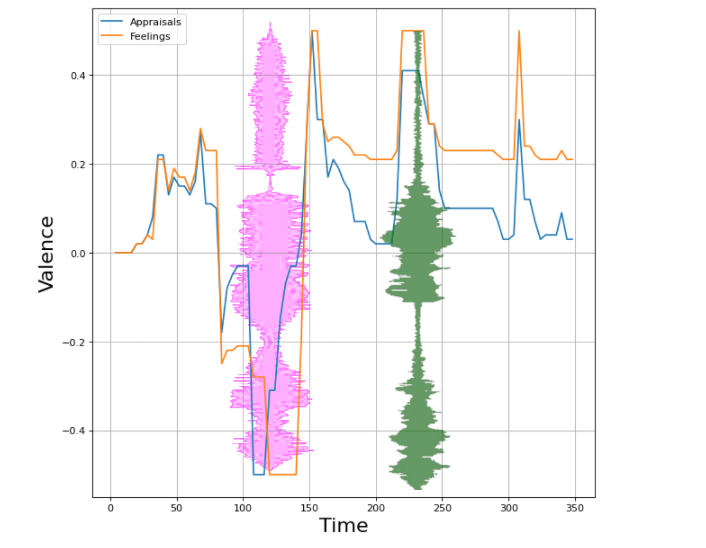
\includegraphics[width=0.75\columnwidth]{./img/GRAFIK.png}
\centering
\caption{Карта перемещений Виртуального Актора и человека}
\label{pic:grafik_res}
\end{figure}

На графике \ref{pic:grafik_res} отображена зависимость Feelings и Appraisals
на шкале Valence от времени, во время эксперимента, по результатам которого 
был построен этот график, было 2 ключевых взаимодействия с испытуемым. Эти
Взаимодействия были классифицированы как отрицательное эмоциональное взаимодействие и положительное.
На графике они изображены рорзовым и зеленым - соответственно.
Из изображения видно, что результат взаимодействия был следующим:
в 110 секунду игровой сессии при было обработано негативное высказывание, что 
оказало влияение на график так что по шкале валентности показатель упал.
Обатное произошло на 231 секунде, когда речевое взаимодействие с виртальным 
вгентом имело позитивный характер.

\section{Выводы}

Было реализовано приложение позволяющее взаимодействовать с виртуальным окружением, в частности с виртуальным актором. 
Были дообучены модели машинного обучения с целью построения эмоционального взаимодействия. 
Для чего в приложение были интегрированы различные технические средства.


\clearpage

\chapter*{Заключение}
\addcontentsline{toc}{chapter}{Заключение}

В ходе работы над НИР был разработан и протестирован с участием испытуемых прототип Виртуального Актора, 
обладающий социально-эмоциональным интеллектом и помещенный в виртуальное окружение, которое создано при помощи графического движка Unity3d, 
была реализована система для анализа речи с выявлением эмоций соответствующим речевым признакам, так же были
в дополнении к вышеуказанной системе, были спроектированы и реализованы методы 
воздействия на виртуального агента, основывающиеся на семантической составляющей речевого контекста.
Данная работа является актуальной поскольку на данный момент эта область находится на начальных этапах 
развития и активной интеграции в различные индустрии.
Созданная и протестированная модель интеллекта затем может быть интегрирована в другие проекты с 
Виртуальным Актором: виртуальный слушатель, виртуальный клоун, виртуальный танцор. 

\begin{enumerate}
    \item Были проанализированы различные когнитивные архитектуры.
    \item Проанализированы методы распознавания речи.
    \item Доработан алгоритм поведения Виртуального Актора.
    \item Унифицирован алгоритм поведения Виртуального Актора.
    \item Был разработан, алгоритм выявления эмоций из человеческой речи.
    \item Добавлено возможность эмоционального взаимодействия с виртуальным актором.
    \item Было Реализован визуальный агент и сцена, используя межплатформенную среду разработки компьютерных игр Unity3d.
\end{enumerate}



%Цель работы была полностью достигнута, и поставленные задачи решены. Результаты
%выполнения ВКР были использованы в программном обеспечении, разрабатываемом на
%предприятии АО "Концерн "Созвездие".


\clearpage

\phantomsection
\addcontentsline{toc}{chapter}{\bibname}	% Добавляем список литературы в оглавление
\printbibliography                        % печать библиографии через BibLaTeX

\addcontentsline{toc}{section}{Список литературы}
%%\begin{thebibliography}{99}

%\bibitem{RCO1} {Ермаков А.Е.  Автоматизация онтологического инжиниринга в системах извлечения знаний из текста. М.: ООО ``ЭР СИ О'', Компьютерная лингвистика и интеллектуальные технологии: труды Международной конференци Диалог'2008, 2008.}


%\bibitem{Troel} {Троелсен Э. Язык программирования C\# 2008  и платформа .Net 3.5  М.: издательство <<Вильямс>>{}, 2010. 1344 с.}


%\bibitem{PBIRCH}{Ashwani Garg, Ashish Mangla, Neelima Gupta, Vasudha Bhatnagar PBIRCH: A scalable parallel clustering algorithm for incremental data. //Proceedings of 10th International Database Engineering and Applications Symposium IDEAS06, 2006}



%\end{thebibliography}


\endrefsection

\clearpage

%\chapter*{Приложения}
%\addcontentsline{toc}{chapter}{Приложения}
%\appendixtocon
%\renewcommand{\appendixname}{Приложение}
\appendix
\renewcommand{\appendixtocname}{Приложения}
\addappheadtotoc
%\titleformat{\chapter}[block]{\centering\normalfont\Large\bfseries}{\chaptername{} \thechapter.}{1ex}{}{}
\renewcommand{\chaptername}{Приложение}
%\renewcommand*\printchaptername{\Large\bfseries\appendixname~}
%\renewcommand{\thechapter}{Приложение \Alph{chapter}}
%\renewcommand{\thechaptertoc}{Приложение \Alph{chapter}}

%\renewcommand{\chaptermark}[1]{\markboth{\chaptername\ \thechapter.\ #1}{}}

%\begin{appendices}

%!!!
%\chapter{Основные правила форматирования}\label{app-format}
%\addcontentsline{toc}{chapter}{}

Текст пояснительной записки должен готовиться для печати на листах формата А4, использоваться должен шрифт с засечками (Roman; обычно --- Times Roman или Times New Roman), 12 или 14 кегль. Размеры полей:

\begin{itemize}
	\item верхнее: 20 мм.
	\item нижнее: 20 мм.
	\item левое: 10 мм.
	\item правое: 25 мм.
\end{itemize}

Нумероваться должны все страницы, начиная с первой (титульной), однако сами номера следует проставлять на страницах, начиная со страницы реферата. Номер следует проставлять внизу страницу (в центре).

Заголовки оформляются тем же шрифтом, что и основной текст (т.е., соответственно, Times Roman или Times New Roman). Для заголовков первого уровня размер шрифта может быть больше размера шрифта основного текста (обычно 14-16).

Все разделы текста: реферат, оглавление, введение, три главы основного
содержания, список литературы, заключение, приложения --- должны снабжаться
содержательным заголовком и начинаться с новой страницы; сами заголовки следует
при этом центрировать (заголовки параграфов и пунктов выравниваются по ширине).
Следует обратить внимание, что заголовки всех разделов, кроме трех основных
глав, регламентированы; заголовки трех основных глав должны быть содержательными
и отражать суть соответствующей главы. Названия типа <<Аналитическая часть>> и <<Теоретическая глава>> --- \textit{недопустимы}.

Текст пояснительной записки может содержать рисунки и таблицы. Все рисунки и
таблицы должны снабжаться номерами и подписями:

\begin{itemize}

	\item нумерация рисунков и таблиц должна быть сквозная (но раздельная, т.к. для рисунков своя, для таблиц --- своя);

	\item в случае большого количества иллюстраций/таблиц, допускается <<вложенная>> нумерация (т.е. таблицу/рисунок можно снабжать составным номером в формате 
	
	$$\langle\mbox{номер главы}\rangle.\langle\mbox{номер внутри главы}\rangle;$$
	
	\item подрисуночная подпись должна располагаться снизу по центру;
	
	\item название таблицы следует помещать над таблицей слева, без абзацного
	отступа в одну строку с ее номером через тире (ГОСТ 7.32-2001, п.6.6.1).

\end{itemize}

Здесь перечислены не все, а лишь основные требования к оформлению. Прочие
требования --- см. соответствующие ГОСТы.

Для того чтобы избежать больших отступов в списках, которые по умолчанию добавляют окружения \texttt{itemize} и \texttt{enumerate}, следует использовать 
\texttt{compactitem} (для маркированных списков) и \texttt{compactenum} (для нумерованных списков) из пакета \texttt{paralist}. 
Например:

\begin{compactitem}
	\item это;
	\item не нумерованный;
	\item список;
	\item без лишних промежутков.
\end{compactitem}

И для нумерованных списков:

\begin{compactenum}[1)]
	\item нумерованные списки;
	\item пакета \texttt{paralist};
	\item еще и удобно настраивать;
	\item (например, менять формат номера).
\end{compactenum}

\noindent или

\begin{compactenum}[a)]
	\item это другой;
	\item нумерованный;
	\item список;
	\item без лишних промежутков;
	\item и с буквенной нумерацией.
\end{compactenum}

А если хочется нумерацию сделать ангоязычной, то нужно использовать окружение \texttt{other\-language} (таким образом: \verb|\begin{otherlanguage}[numerals=latin]{russian}|)

\setkeys{russian}{numerals=latin}
%\selectlanguage{russian}
%\begin{otherlanguage}[numerals=latin]{russian}
\begin{russian}
\begin{compactenum}[a)]
	\item это другой;
	\item нумерованный;
	\item список;
	\item без лишних промежутков;
	\item и с буквенной нумерацией.
\end{compactenum}
\end{russian}
%\end{otherlanguage}

\textbf{Замечание.} По неизвестным причинам, переключения не происходит, хотя должно.

%\clearpage

%\chapter{Общая структура пояснительной записки}\label{app-structure}
%\addcontentsline{toc}{chapter}{}

\refsection

\begin{enumerate}
	\item Титульный лист %(в данном примере используется титульный лист от преддипломной практики)
	\item Лист с подписями (только для ВКР)
	\item Задание (в данном примере используется задание на диплом)
	\item Отчет из Интиплагиага \footnote{Обычно, допускается до 30\% заимствованного текста для работ бакалавров и до 20\% -- для работ магистров; см. соответствующие нормативные документы}
	\item Реферат (всегда на отдельной стр.)%, и эта страница \textit{НЕ} нумеруется)
	\item Оглавление. Начинается с новой страницы. %Обычно, это первая нумеруемая страница.
	\item Введение
	\begin{enumerate}
		\item Актуальность
		\item Новизна
		\item Оригинальная суть исследования
		\item Содержание ПЗ по главам (тезисно)
	\end{enumerate}
	\item Аналитическая глава. Пишется в стиле \textit{аналитического обзора}
	\item Теоретическая и инженерная глава. Описываются использованные, доработанные и разработанные модели, алгоритмы, методы, и т.п. Кроме того, тут формулируется архитектура системы.
	\item Инженерная глава. В этой главе следует отразить результаты проектирования, что, в общем случае, включает в себя следующие пункты:
	\begin{enumerate}
		\item Описание используемой методики проектирования
		\item Общая архитектура системы
		\item Архитектура подсистемы [таких подразделов может быть несколько штук, по одному на каждую подсистему или модуль, требующую детальное рассмотрение]
		\item Проектирование внешних и внутренних интерфейсов/протоколов взаимодействия
	\end{enumerate}
	\item Практическая глава. Описывается реализация, включая выбор инструментальных средств \footnote{В тех случаях, когда \begin{inparaenum}[(a)]\item этот выбор имеет существенное значение для всей работы и \item он не был, по каким-либо причинам, проделан в аналитической главе \end{inparaenum}}. Типовое содержание:
	\begin{enumerate}
		\item Состав и структура реализованного ПО 
		\item Выбор инструментальных средств
		\item Основные сценарии работы различных категорий пользователей
		\item Результаты тестирования (разработка тестовых примеров, таблицы и графики результатов прогона)
		\item Сравнение с существующими аналогами
	\end{enumerate}
	\item Заключение
	\item Список литературы 
	\item Приложения
\end{enumerate}

Кроме того, в ПЗ могут включаться и такие разделы, как словарь терминов, 
список сокращений и др. В зависимости от предпочтений автора, могут 
помещаться как в начале ПЗ (до оглавления), так и в конце (после заключения, 
но до приложений).

\paragraph{Замечания}: \mynobreakpar %\nopagebreak

\begin{enumerate}

  \item На каждый элемент из списка литературы должна быть хотя
бы одна ссылка в тексте.

  \item Список литературы должен быть оформлена согласно ГОСТ
\cite{Gost.7.1.2003,Gost.7.0.5.2008}.

  \item Минимальное количество источников для УИРов --- 15--20 (для
работ с большой аналитической и теоретической частью нормальное количество ---
25-30 и более), для дипломов --- соответственно, 30--35 и 35--60. Эти цифры
существенны, т.к. <<недобор>>, как правило, свидетельствует о не выполнении
аналитической части работы и, следовательно, недостаточном владении предметом.

  \item При подготовке РСПЗ рекомендуется вставлять уже наработанные к 
моменту подготовки РСПЗ материалы. Однако, в любом случае, каждый раздел 
должен начинаться с аннотации, заключенной в окружение \verb|\annotation|. В 
пояснительной записке к диплому аннотации не нужны. 

  \item Между заголовком главы и первым разделом рекомендуется поместить один-два абзаца связанного текста с кратким содержанием (планом) главы.

  \item Общее число и объем приложений не ограничивается. Объем ПЗ
\textbf{\textit{без}} приложений --- 25--40 стр. для УИРов, и не менее 60--100
стр. для дипломов. Объем ПЗ не может быть меньше указанных размеров. Это
означает, что студент не выполнил работу, или, как минимум, не удосужился
подготовить адекватную ПЗ. Превышать верхние пределы также не желательно, в
некоторых комиссиях это может восприниматься негативно; однако, в целом,
небольшое превышение допустимо, если проделана действительно большая работа и
получено много результатов (например, экспериментальных, или получены
нетривиальные аналитические или теоретические результаты).

  \item ГОСТ требует, чтобы нумерация страниц начиналась с 
первой, титульной, страницы. При этом на самой титульной странице номер не 
печатается. В данном случае, номера также не проставляются на листах задания, 
а также на листе с подписями (для ВКР).

\end{enumerate}

\printbibliography[heading=subbibliography]

\endrefsection


%\clearpage

%\chapter{Правила использования шаблона}\label{app-manual}

Настоящий шаблон все еще несколько несовершенен в плане оформления: например, неправильная нумерация приложений, и еще несколько нюансов. В последующих версиях это будет исправляться.

Ниже описана структура исходных текстов шаблона (и, соответственно, структура исходных текстов ПЗ).

Кодировка всех файлов — UTF8, и для сборки PDF документов следует использовать команду \texttt{xelatex}.

Головной файл --- \texttt{thesis-template.tex}. Его задача --- <<склеить>> вместе разные части ПЗ. Каждая часть (реферат, введение, каждая содержательная глава, заключение, библиография, приложения) выделяется в отдельный файл. 

\begin{itemize}
  \item[] \texttt{thesis-macro.tex} --- содержит определения различных макрокоманд, которые часто используются в конкретной работе, например, определения окружения для теорем, некоторые часто используемые формулы, и т.п.;
  \item[] \texttt{thesis-abstract.tex} --- содержит аннотацию;
  \item[] \texttt{thesis-intro.tex} --- содержит введение;
  \item[] \texttt{thesis-chapter1.tex} --- текст первой главы;
  \item[] \texttt{thesis-chapter2.tex} --- текст второй главы;
  \item[] \texttt{thesis-chapter3.tex} --- текст третьей главы;
  \item[] \texttt{thesis-bibl.tex} --- список литературы (только подключение к
  проекту);
  \item[] \texttt{biblio.bib} --- собственно библиография (в формате BibTeX);
  \item[] \texttt{thesis-conclusion.tex} --- заключение;
  \item[] \texttt{thesis-appendix1.tex} --- первое приложение;
  \item[] \texttt{thesis-appendix2.tex} --- второе приложение;
\end{itemize}


%Одна из первых вещей, которые необходимо сделать при использовании данного шаблона --- это отредактировать аргумент команды \verb|\headertext| в начале головного файла.

Головной файл нужно менять лишь тогда, когда нужно добавить в проект новый файл,
или удалить существующий (см. команду \verb|\input|). Обычно, это требуется,
когда нужно добавить/удалить приложения.

\section{Титульные листы}

Существует два варианта генерации титульных листов:

\begin{itemize}
  \item использование листов, сверстанных в \LaTeX{} (используется по
  умолчанию);
  \item подстановка пустых бланков из PDF-файлов.
\end{itemize}

\subsection{Титульные листы LaTeX}

Проект содержит определения титульных листов, описанные в виде \textbf{.tex}
файлов. На данный момент требуется заполнение данных студента вручную. Позже
будет реализована автоматическая подстановка данных проекта при инициализации
репозитория.

\subsection{Титульные листы из PDF}

При возникновении проблем с использованием титульных листов \LaTeX{} возмодно
включить в документ бланки титульных листов из PDF-файлов. Для этого нужно
раскомментировать соответствующие команды \textbf{includepdf} в начале
документа.

Для того, чтобы \LaTeX{} при компиляции автоматически <<подхватил>> задание, его
нужно сохранить в формате pdf (например, с помощью вирутального принтера),
поместить в ту же папку \texttt{/title} и назвать \texttt{task.pdf}. Точно также
следует поступить с титульной страницей (\texttt{title.pdf}). При оформлении ПЗ
для ВКР следует дополнительно поместить в папку \texttt{/title} pdf-версию листа
с подписями, назвав файл \texttt{title-dep22.pdf}. После этого нужно
раскомментировать команду
\begin{center}
  \verb|\includepdf[ ... ]{title/title-dep22.pdf}|
\end{center}
в начале головного файла.

Образцы и Word-шаблоны титульных листов для (РС)ПЗ к УИРам, НИРам, практикам и
ВКР доступны в репозитории
\begin{center}
  \url{https://gitlab.com/skibcsit/thesis-titles}.
\end{center}  

\textbf{Замечание}. В шаблоне используется пакет \texttt{hyperref}, который
делает две вещи: все перекрестные ссылки <<кликабельны>>, а также выделены
(красной) рамочкой. Эти рамки \textit{не выводятся на печать}. Вместо цветных
рамок, возможны другие способы выделения ссылок (см. документацию пакета).

%!!!

%\end{appendices}

\end{document}



